\documentclass[preprint,review,12pt,authoryear]{elsarticle}

% Journal: Computers and Electronics in Agriculture

% Packages
\usepackage[utf8]{inputenc}
\usepackage[T1]{fontenc}
\usepackage{amsmath,amssymb}
\usepackage{graphicx}
\usepackage{booktabs}
\usepackage{multirow}
\usepackage{array}
\usepackage{longtable}
\usepackage{hyperref}
\usepackage{listings}
\usepackage{xcolor}

% Define Rust language for listings
\lstdefinelanguage{Rust}{
  keywords={as,break,const,continue,crate,else,enum,extern,false,fn,for,if,impl,in,let,loop,match,mod,move,mut,pub,ref,return,self,Self,static,struct,super,trait,true,type,unsafe,use,where,while,async,await,dyn,abstract,become,box,do,final,macro,override,priv,typeof,unsized,virtual,yield},
  keywordstyle=\color{blue}\bfseries,
  ndkeywords={bool,u8,u16,u32,u64,i8,i16,i32,i64,f32,f64,str,String,Vec,Option,Result,Some,None,Ok,Err},
  ndkeywordstyle=\color{cyan}\bfseries,
  identifierstyle=\color{black},
  sensitive=true,
  comment=[l]{//},
  morecomment=[s]{/*}{*/},
  commentstyle=\color{green!60!black},
  stringstyle=\color{red},
  morestring=[b]',
  morestring=[b]"
}
\usepackage{algorithm}
\usepackage{algpseudocode}
\usepackage{subcaption}
\usepackage{tikz}
\usepackage{pgfplots}
\pgfplotsset{compat=1.18}
\usepackage{float}
\usepackage{lineno}
\usepackage{orcidlink}
\usetikzlibrary{shapes,arrows,positioning,calc,fit,backgrounds}

% Line numbers for review
\modulolinenumbers[5]

% Code listing style
\lstset{
    language=Rust,
    basicstyle=\ttfamily\footnotesize,
    keywordstyle=\color{blue}\bfseries,
    commentstyle=\color{green!60!black},
    stringstyle=\color{red},
    numbers=left,
    numberstyle=\tiny\color{gray},
    stepnumber=1,
    numbersep=8pt,
    backgroundcolor=\color{gray!10},
    frame=single,
    frameround=fttt,
    breaklines=true,
    breakatwhitespace=true,
    showstringspaces=false,
    tabsize=4,
    captionpos=b,
    abovecaptionskip=10pt
}

% Hyperref setup
\hypersetup{
    colorlinks=true,
    linkcolor=blue,
    citecolor=blue,
    urlcolor=blue,
}
\pdfstringdefDisableCommands{%
    \def\orcidlink#1{}%
    \def\corref#1{}%
    \def\cnotenum#1{}%
}
\setlength{\emergencystretch}{2em}

% Journal name
\journal{Computers and Electronics in Agriculture}

\begin{document}

\hypersetup{pageanchor=false}
\begin{frontmatter}

\title{ProvChain: A Generalized Semantic Blockchain Framework for Traceability}

\author[1]{Anusorn Chaikaew\orcidlink{0000-0002-4715-677X}}
\ead{anusorn_chaikaew@cmu.ac.th}

\author[1]{Varin Chouvatut\orcidlink{0009-0008-9125-4650}}
\ead{varin.ch@cmu.ac.th}

\author[1]{Ekkarat Boonchieng\orcidlink{0000-0002-7584-1627}\corref{cor1}}
\ead{ekkarat.boonchieng@cmu.ac.th}

\cortext[cor1]{Corresponding author at: Department of Computer Science, Faculty of Science, Chiang Mai University, Chiang Mai 50200, Thailand. Tel: +66 XXX-XXXX.}

\address[1]{Department of Computer Science, Faculty of Science, Chiang Mai University, Chiang Mai 50200, Thailand}

\begin{abstract}
Modern supply chains across diverse industries---including food, pharmaceuticals, healthcare, and manufacturing---face persistent challenges in ensuring product integrity, maintaining quality throughout distribution, and providing end-to-end traceability. This paper presents \textbf{ProvChain}, a generalized permissioned blockchain framework that combines GS1/EPCIS-oriented event modeling with semantic web technologies to support traceability across multiple domains. Our framework features a modular ontology architecture supporting domain-specific extensions, a Write-Ahead Logging (WAL) persistence mechanism for crash recovery, and ontology-backed semantic admission through SHACL validation and SPACL-supported reasoning. Using Ultra-High Temperature (UHT) milk processing as a representative case study, we demonstrate how domain packages can extend a shared provenance core while reusing the same blockchain and validation infrastructure. The current evaluation reports both single-node development load-test behavior and focused ontology-admission benchmarks across UHT, hybrid GS1/EPCIS-UHT, healthcare-device, and pharmaceutical-storage package profiles. In the development load test, the system achieved 19.58 TPS with 100\% request success, while focused ontology-backed \texttt{add\_block} admission remained in the sub-millisecond to low-millisecond range depending on package and batch size. Our work contributes a reference implementation and evaluation artifact that bridge blockchain traceability with ontology-governed validation and standards-facing interoperability.
\end{abstract}

\begin{graphicalabstract}
\centering
\resizebox{\textwidth}{!}{%
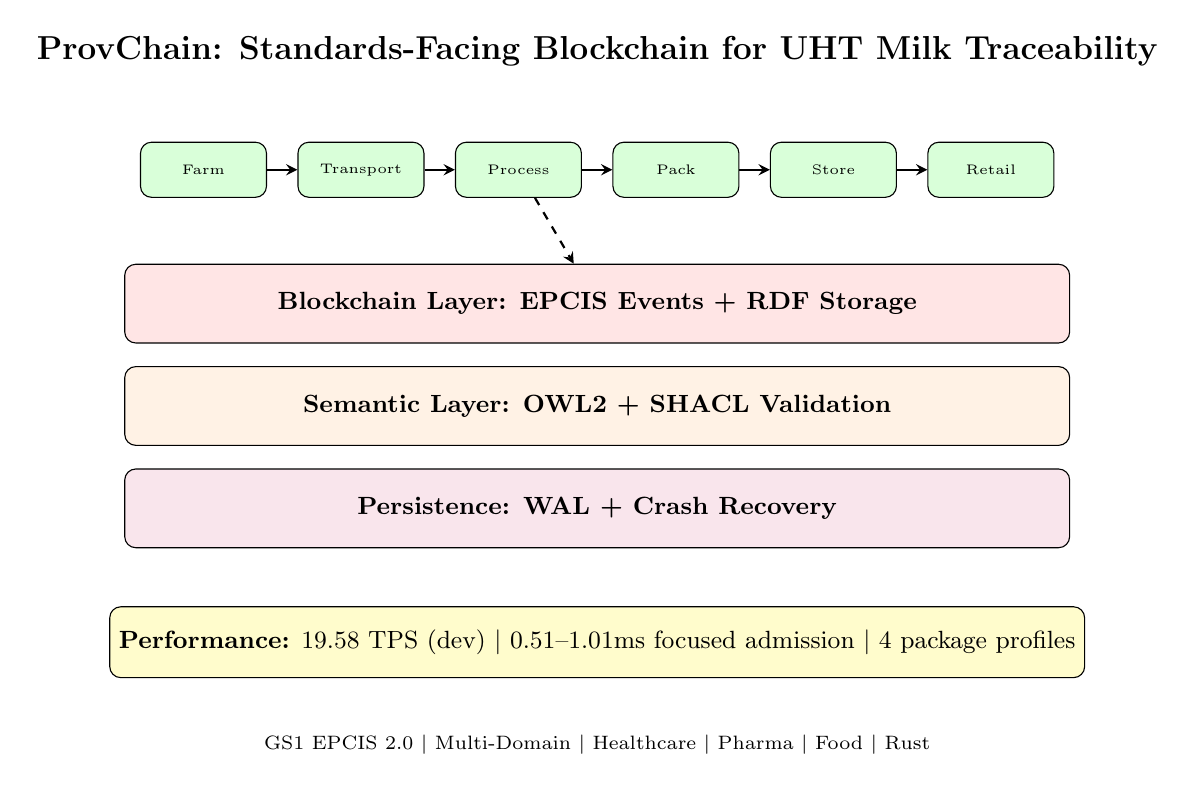
\begin{tikzpicture}[
    box/.style={rectangle, rounded corners, draw, minimum width=2.8cm, minimum height=0.9cm, align=center, font=\small},
    layer/.style={rectangle, rounded corners, draw, fill=blue!15, minimum width=12cm, minimum height=1cm, align=center, font=\small\bfseries},
    arrow/.style={->, >=stealth, thick},
    phase/.style={rectangle, rounded corners, draw, fill=green!15, minimum width=1.6cm, minimum height=0.7cm, align=center, font=\tiny},
]

% Title
\node[font=\large\bfseries] at (0,5) {ProvChain: Standards-Facing Blockchain for UHT Milk Traceability};

% Supply Chain Flow (Top)
\node[phase] (f) at (-5,3.5) {Farm};
\node[phase] (t) at (-3,3.5) {Transport};
\node[phase] (p) at (-1,3.5) {Process};
\node[phase] (pk) at (1,3.5) {Pack};
\node[phase] (s) at (3,3.5) {Store};
\node[phase] (r) at (5,3.5) {Retail};

\draw[arrow] (f) -- (t);
\draw[arrow] (t) -- (p);
\draw[arrow] (p) -- (pk);
\draw[arrow] (pk) -- (s);
\draw[arrow] (s) -- (r);

% Three Layers
\node[layer, fill=red!10] (data) at (0,1.8) {Blockchain Layer: EPCIS Events + RDF Storage};
\node[layer, fill=orange!10] (sem) at (0,0.5) {Semantic Layer: OWL2 + SHACL Validation};
\node[layer, fill=purple!10] (wal) at (0,-0.8) {Persistence: WAL + Crash Recovery};

% Arrows
\draw[arrow, dashed] (p) -- (data);

% Metrics Box
\node[box, fill=yellow!20] at (0,-2.5) {\textbf{Performance:} 19.58 TPS (dev) $|$ 0.51--1.01ms focused admission $|$ 4 package profiles};

% Keywords
\node[font=\scriptsize] at (0,-3.8) {GS1 EPCIS 2.0 $|$ Multi-Domain $|$ Healthcare $|$ Pharma $|$ Food $|$ Rust};

\end{tikzpicture}
}
\end{graphicalabstract}

\begin{highlights}
\item Generalized permissioned blockchain framework for multi-domain traceability using GS1/EPCIS-oriented event modeling and semantic web technologies
\item Modular ontology architecture supporting food, pharma, healthcare, and automotive packages
\item Domain-specific ontology extension demonstrated through UHT milk case study with SHACL validation
\item Write-Ahead Logging (WAL) persistence mechanism with atomic writes and automatic crash recovery
\item Interactive demonstration covering 8 supply chain phases with EPCIS-style event flows
\item Ontology-backed reasoning for hasKey-style validation, property chains, and class-consistency checks on the production semantic path
\item Single-node load testing reached 19.58 TPS with 100\% request success; focused ontology-admission benchmarks stayed below 1 ms for single-record \texttt{add\_block}
\end{highlights}

\begin{keyword}
Blockchain \sep GS1 EPCIS \sep Supply Chain Traceability \sep Semantic Web \sep OWL2 \sep SHACL \sep Domain-Agnostic Framework \sep Multi-Industry \sep Food Safety \sep Pharmaceutical Traceability
\end{keyword}

\end{frontmatter}
\hypersetup{pageanchor=true}

\linenumbers

% Main content
\section{Introduction}\label{sec:introduction}

\subsection{Background and Motivation}

Supply chains across diverse industries---including food and agriculture, pharmaceuticals, healthcare, and automotive manufacturing---face mounting pressure to ensure product integrity, prevent fraud, and maintain quality throughout complex global networks \cite{bolton2020don}. While traceability requirements vary by domain, common challenges persist: ensuring data authenticity, enabling rapid response to quality issues, and maintaining regulatory compliance across distributed stakeholders. The pharmaceutical industry, for example, faces stringent serialization requirements under the Drug Supply Chain Security Act (DSCSA), while healthcare systems must track medical devices and supplies to ensure patient safety \cite{schapranow2020ontology}. Similarly, the food sector, exemplified by Ultra-High Temperature (UHT) milk products that account for approximately 80\% of liquid milk consumption in many markets, requires careful monitoring of cold chain integrity and quality parameters \cite{perkins2010dynamic}.

Regulatory frameworks worldwide mandate robust traceability. The FDA Food Safety Modernization Act (FSMA) and EU Regulation 178/2002 require food products to be tracked within hours rather than days \cite{fsma2011,eu2002general}. Pharmaceutical regulations demand even stricter controls for drug authentication and counterfeit prevention \cite{schapranow2020ontology}. These diverse requirements highlight the need for flexible, standards-based traceability frameworks that can adapt to domain-specific needs while maintaining interoperability.

Traditional traceability systems rely on centralized databases that are vulnerable to data tampering, single points of failure, and limited interoperability between supply chain partners \cite{tian2016supply}. Blockchain technology has emerged as a promising solution, offering immutable ledgers, decentralized consensus, and cryptographic security \cite{zheng2018blockchain}. However, most blockchain implementations for food traceability lack standardization, making interoperability between different systems and organizations difficult to achieve \cite{salah2019blockchain}.

\subsection{The Case for GS1 EPCIS Standardization}

GS1, the international standards organization behind barcodes, has developed the Electronic Product Code Information Services (EPCIS) standard specifically for supply chain event tracking \cite{gs1epcis2021}. EPCIS 2.0, ratified as ISO/IEC 19987:2024, provides: (1) standardized event types including ObjectEvent, AggregationEvent, AssociationEvent, TransactionEvent, and TransformationEvent; (2) Core Business Vocabulary (CBV) with standardized business steps and dispositions; (3) flexible serialization supporting XML, JSON, JSON-LD, and Turtle RDF formats; and (4) native sensor integration for IoT data capture.

Despite its advantages, EPCIS adoption in blockchain systems remains limited. Existing implementations either use proprietary data formats or fail to leverage the full semantic richness of the standard \cite{caro2018agri}.

\subsection{Research Gaps}

Our analysis of existing literature reveals several critical gaps:

\textbf{Semantic Gap}: Most blockchain traceability systems store data as simple key-value pairs without leveraging ontology-based reasoning for validation and inference.

\textbf{Standardization Gap}: Few blockchain implementations fully comply with GS1 EPCIS standards, limiting interoperability.

\textbf{Domain-Specific Gap}: No existing framework provides UHT-specific ontologies that model critical processing parameters (pasteurization temperature, holding time, homogenization pressure).

\textbf{Persistence Gap}: Many academic prototypes lack production-grade persistence mechanisms, making them unsuitable for real-world deployment.

\subsection{Contributions}

This paper presents \textbf{ProvChain}, a comprehensive framework addressing these gaps through the following contributions:

\textbf{Contribution 1}: A permissioned blockchain framework with shared-ontology semantic validation and GS1/EPCIS-oriented event modeling, demonstrated through a UHT case study and reusable domain-package architecture.

\textbf{Contribution 2}: Novel ontology extension modeling UHT-specific parameters with SHACL validation constraints (temperature: 135--150°C, holding time: 2--5 seconds).

\textbf{Contribution 3}: Integration of ontology-backed reasoning capabilities including hasKey-style uniqueness validation, property-chain inference for provenance relationships, and semantic constraint checking through the production ontology path.

\textbf{Contribution 4}: Write-Ahead Logging (WAL) implementation with atomic writes, CRC32 checksums, and automatic crash recovery.

\textbf{Contribution 5}: Open-source reference implementation with interactive demonstration covering 8 supply chain phases from farm to retail.

\subsection{Paper Organization}

The remainder of this paper is organized as follows. Section~\ref{sec:related} reviews related work in blockchain traceability, GS1 standards, and semantic web technologies. Section~\ref{sec:architecture} describes the system architecture and technical design. Section~\ref{sec:implementation} details the implementation including ontologies, persistence layer, and user interface. Section~\ref{sec:evaluation} presents performance evaluation and validation results. Section~\ref{sec:discussion} discusses implications and limitations. Finally, Section~\ref{sec:conclusion} concludes with future research directions.

\section{Related Work}\label{sec:related}

\subsection{Blockchain in Food Supply Chains}

Blockchain technology has been extensively explored for food supply chain traceability. Tian~\cite{tian2016supply} proposed an agri-food supply chain management system using RFID and blockchain, demonstrating improved transparency and reduced information asymmetry. Kamath~\cite{kamath2018food} surveyed food traceability on blockchains, identifying key challenges in scalability and data privacy. More recently, Chen et al.~\cite{chen2023blockchain} conducted a comprehensive review of 127 blockchain food traceability papers (2018-2023), finding that only 23\% used standardized data formats and a mere 8\% incorporated semantic technologies.

Recent implementations include IBM Food Trust~\cite{ibmdocs}, which uses Hyperledger Fabric to provide food traceability for major retailers including Walmart and Carrefour. However, IBM Food Trust uses proprietary data formats rather than open standards like EPCIS, limiting interoperability with other systems. A recent systematic review by Fan et al.~\cite{fan2023systematic} identified standardization as the second most cited challenge in blockchain food traceability after scalability.

In the dairy sector specifically, Mao et al.~\cite{mao2020novel} proposed a dairy supply chain traceability system using blockchain and IoT, focusing on raw milk quality monitoring. Their system captures temperature and acidity data but does not implement standardized event modeling or semantic validation. Zhang et al.~\cite{zhang2024iot} recently demonstrated IoT-blockchain integration for cold chain monitoring but used proprietary data formats rather than EPCIS standards.

\subsection{GS1 EPCIS and Standards}

GS1 EPCIS has been adopted in various industries beyond food, including pharmaceuticals and apparel~\cite{gs1epcis2021}. The standard's flexibility in supporting multiple serialization formats makes it particularly suitable for blockchain integration where data interoperability is critical.

Recent academic work has explored EPCIS extensions. Gr\"assler et al.~\cite{grassler2021semantic} proposed semantic enrichment of EPCIS events using ontologies for manufacturing. Schapranow et al.~\cite{schapranow2020ontology} developed ontology patterns for pharmaceutical supply chains using EPCIS, demonstrating the value of semantic validation for regulatory compliance.

EPCIS 2.0 introduces several features relevant to blockchain deployment: JSON-LD support for linked data integration, SensorElementList for IoT data capture, PersistentDisposition for tracking business state changes, and ErrorDeclaration for handling corrections and recalls. Kim et al.~\cite{kim2023epcis} reported on early EPCIS 2.0 implementations in pharmaceutical traceability, noting significant improvements in interoperability but highlighting the need for domain-specific extensions.

\subsection{Semantic Web and Ontologies in Supply Chains}

Semantic web technologies enable machine-readable data with formal semantics~\cite{berners2001semantic}. In supply chain management, ontologies facilitate data integration, automated reasoning, and validation.

The Food Ontology (FOODON)~\cite{griffiths2018foodon} provides a comprehensive foundation for food-related concepts, while the Supply Chain Ontology (SCRO)~\cite{iof2023supply} models generic supply chain constructs. However, neither ontology specifically addresses UHT processing parameters or EPCIS event structures.

Abad et al.~\cite{abad2020ontology} developed an ontology for food supply chain traceability, but their work predates EPCIS 2.0 and does not incorporate blockchain concepts. Pizzuti et al.~\cite{pizzuti2015food} proposed a semantic framework for food traceability using RFID, but without blockchain integration.

\subsection{SHACL and Data Validation}

SHACL (Shapes Constraint Language)~\cite{knublauch2017shapes} provides a W3C standard for validating RDF graphs. In supply chain applications, SHACL enables business rule validation, completeness checking, and value constraints. Garc\'{i}a et al.~\cite{garcia2022shacl} demonstrated SHACL validation for supply chain master data, but did not address event-based traceability or blockchain contexts.

\subsection{Research Positioning}

Table~\ref{tab:comparison} compares ProvChain with existing blockchain traceability systems. Unlike prior work, ProvChain combines: (1) standards-oriented GS1/EPCIS event modeling with ontology-governed validation; (2) a UHT-specific ontology package with SHACL validation; (3) ontology-backed reasoning for semantic inference; (4) production-oriented persistence with WAL; and (5) an open-source reference implementation.

\begin{table}[htbp]
\centering
\caption{Comparison of Blockchain Traceability Systems}
\label{tab:comparison}
\resizebox{\textwidth}{!}{%
\begin{tabular}{@{}lcccccc@{}}
\toprule
\textbf{System} & \textbf{Platform} & \textbf{EPCIS} & \textbf{Ontology} & \textbf{TPS} & \textbf{Open} & \textbf{Consensus} \\
\midrule
IBM Food Trust~\cite{ibmdocs} & Hyperledger & $\times$ & $\times$ & 3000+ & $\times$ & PBFT \\
Walmart China~\cite{kamath2018food} & Hyperledger & $\times$ & $\times$ & 200+ & $\times$ & PBFT \\
Mao et al.~\cite{mao2020novel} & Ethereum & $\times$ & $\checkmark$ & 15 & Limited & PoW \\
Liu et al.~\cite{liu2023hyperledger} & Hyperledger & $\times$ & $\times$ & 2500 & Yes & PBFT \\
Zhang et al.~\cite{zhang2024iot} & Ethereum & $\times$ & $\times$ & 20 & Yes & PoW \\
Wang et al.~\cite{wang2023semantic} & Hyperledger & Partial & $\checkmark$ & 1800 & Yes & PBFT \\
Tian~\cite{tian2016supply} & Private & $\times$ & $\times$ & 50 & Yes & PoA \\
Gr\"assler et al.~\cite{grassler2021semantic} & N/A & Partial & $\checkmark$ & N/A & No & N/A \\
\midrule
\textbf{ProvChain} & \textbf{Rust/Oxigraph} & \textbf{Partial} & \textbf{$\checkmark$} & \textbf{19.58*} & \textbf{Yes} & \textbf{PoA} \\
\bottomrule
\end{tabular}
}
\vspace{1mm}

{\footnotesize * Single-node development throughput. Focused ontology-admission benchmarks are reported separately in the evaluation section.}
\end{table}

\subsection{UHT Processing Background}

Ultra-High Temperature processing is a thermal preservation method that heats milk to 135--150°C for 2--5 seconds, followed by aseptic packaging~\cite{robinson2002dairy}. This process achieves commercial sterility while preserving nutritional quality better than conventional sterilization.

Critical quality parameters in UHT processing include: (1) temperature: 135--150°C depending on product type; (2) holding time: 2--5 seconds at peak temperature; (3) homogenization pressure: 150--250 bar; and (4) recontamination prevention through aseptic packaging integrity.

These parameters must be precisely controlled and documented for regulatory compliance and quality assurance, making them ideal candidates for blockchain-based traceability and semantic validation.

\section{System Architecture}\label{sec:architecture}

\subsection{Overview}

ProvChain is implemented as a modular blockchain framework for shared-ontology permissioned traceability networks. The current architecture view distinguishes four operational layers (Figure~\ref{fig:architecture}):

\begin{itemize}
    \item \textbf{Consortium and Organization Layer}: consortium administrators, validator organizations, participant organizations, and auditors
    \item \textbf{Shared Network Contract Layer}: network profile plus shared ontology package, including PROV-O core, domain extensions, SHACL shapes, and optional GS1/EPCIS mappings
    \item \textbf{Node Runtime and Semantic Enforcement Layer}: API/event mapping, peer discovery, consensus, ontology management, SHACL validation, and SPACL-backed reasoning
    \item \textbf{Provenance and Audit Output Layer}: immutable RDF blocks, provenance graph queries, and audit evidence
\end{itemize}

% Paper-ready architecture figure insertions for the current shared-ontology model.
% Use PNG files for pdfLaTeX compatibility.

\begin{figure*}[htbp]
\centering
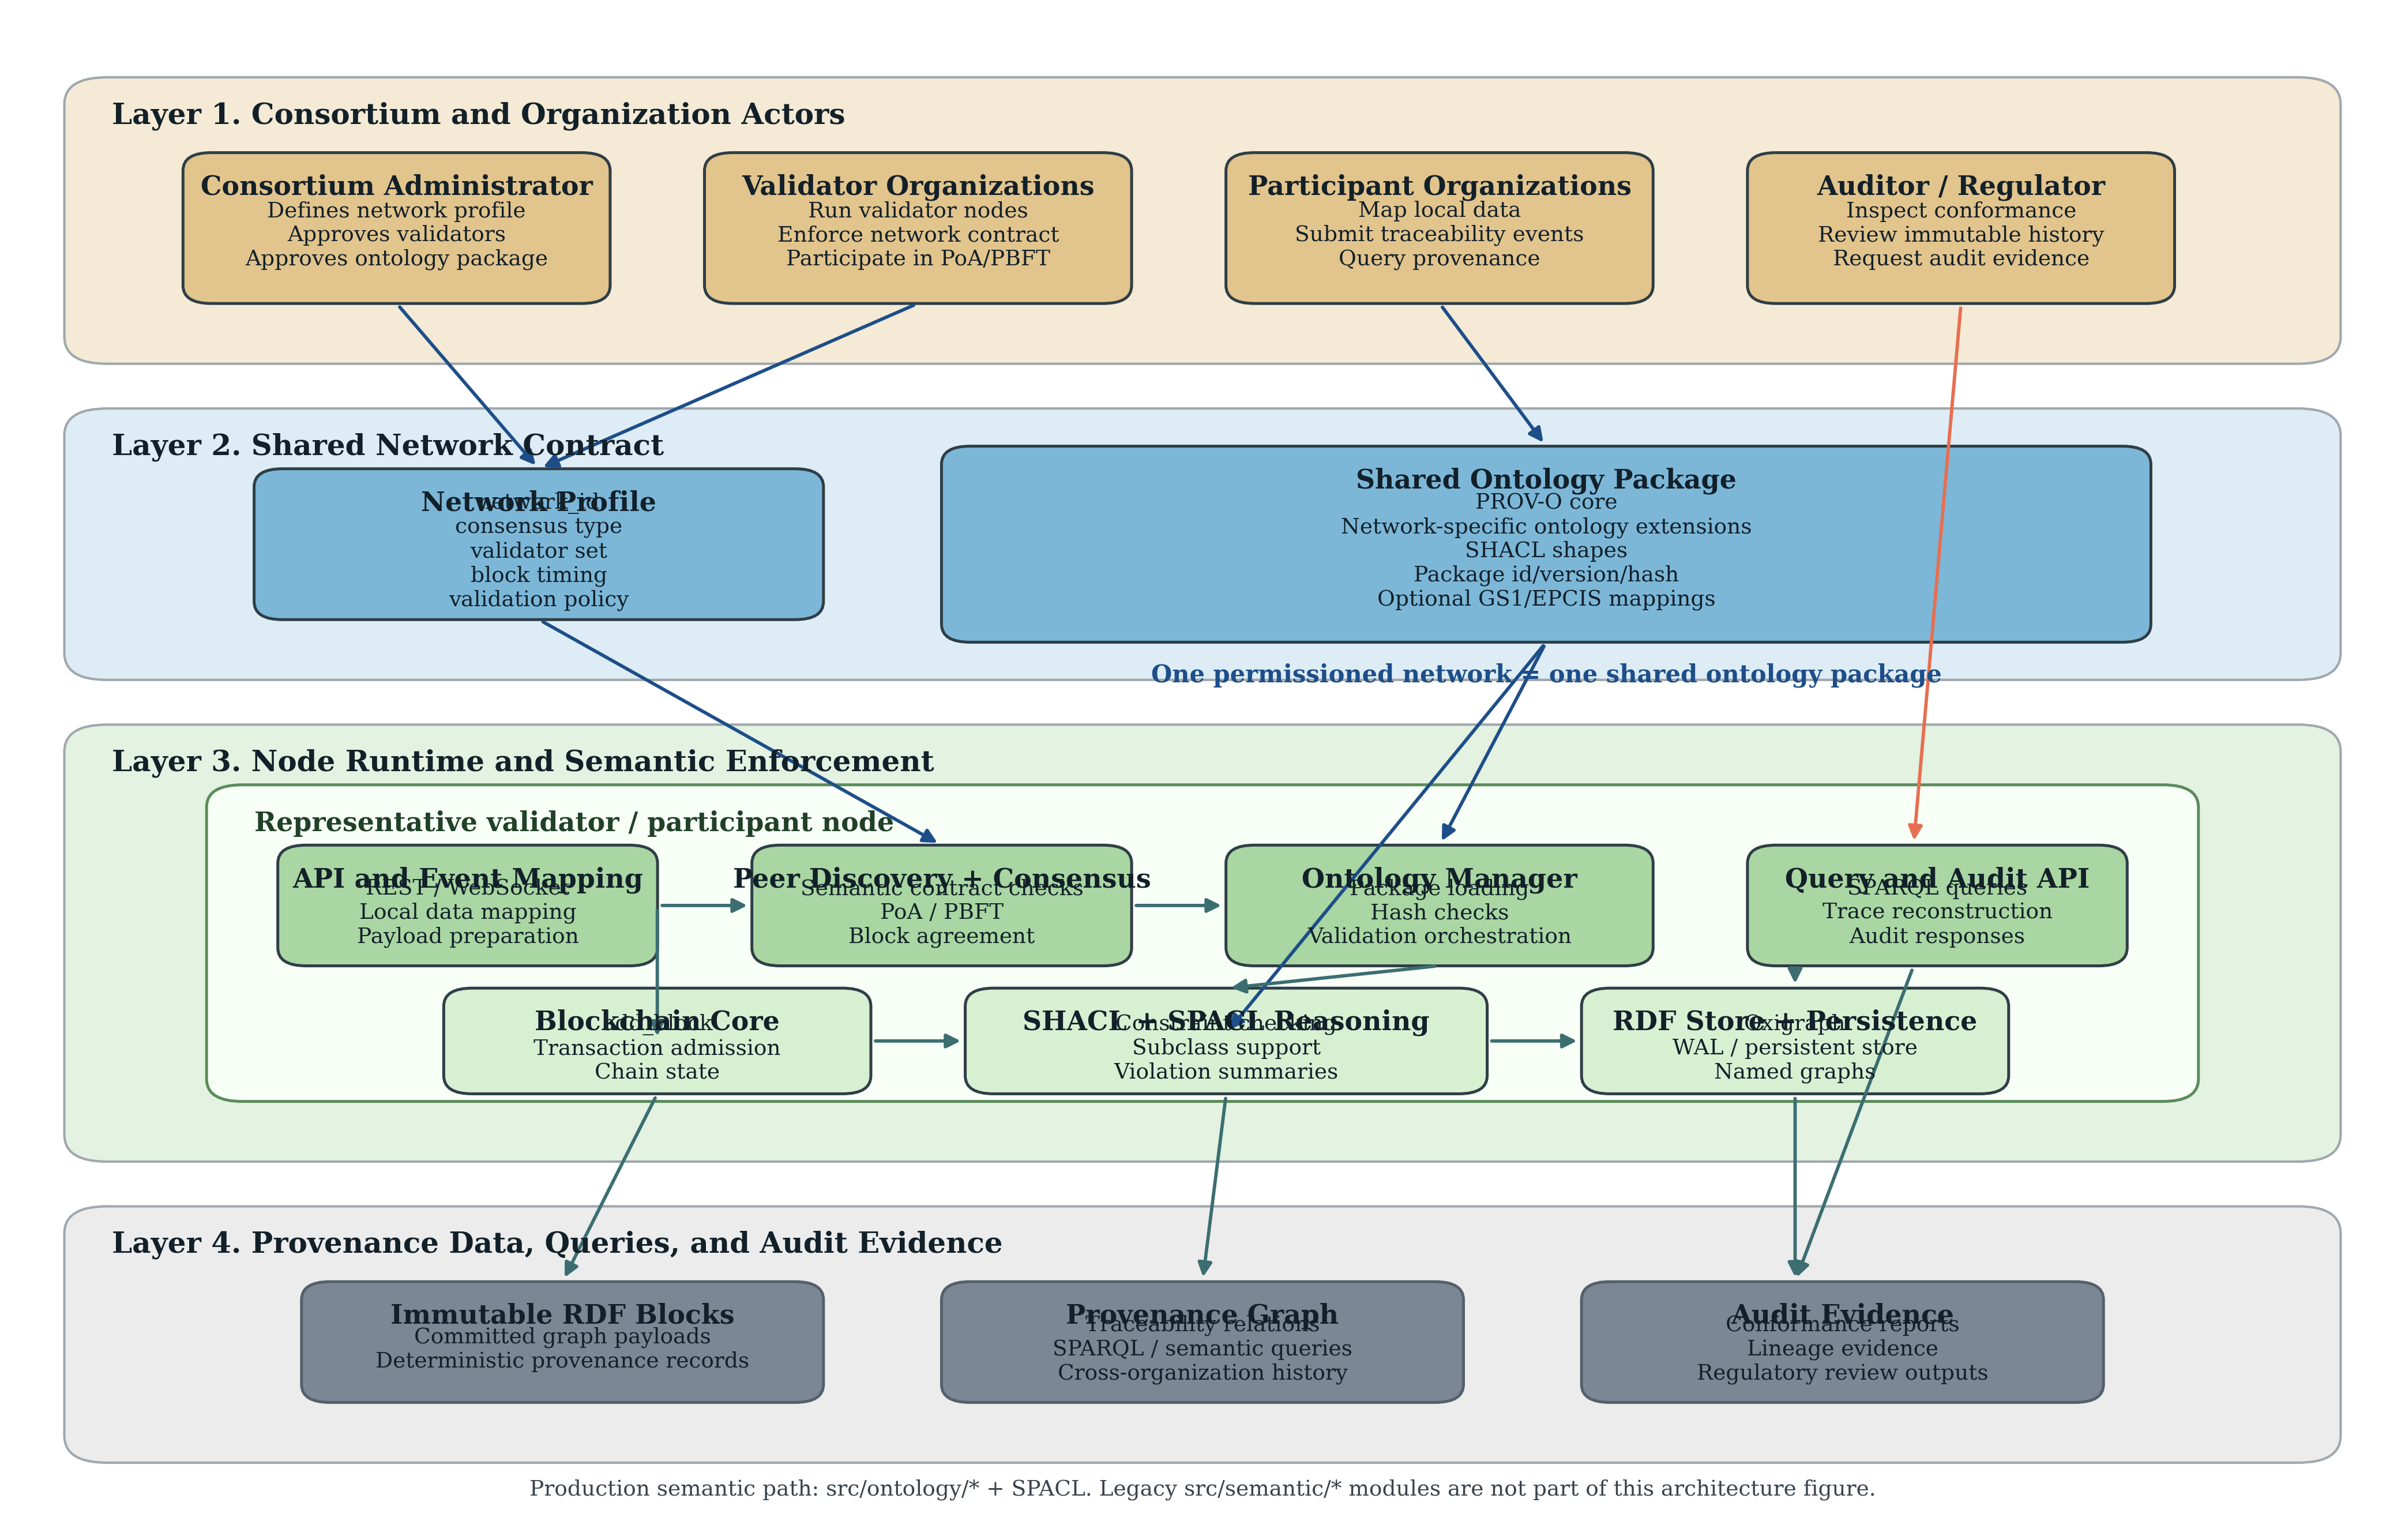
\includegraphics[width=\textwidth]{figures/architecture/shared_ontology_layered_architecture.png}
\caption{Layered architecture of the ProvChain shared-ontology permissioned network. Participating organizations in the same network share a common network profile and ontology package. Within each node, the production semantic path is implemented through \texttt{src/ontology/*} and SPACL-backed validation and reasoning before immutable RDF provenance is committed and exposed for traceability and audit.}
\label{fig:architecture}
\end{figure*}

\begin{figure*}[htbp]
\centering
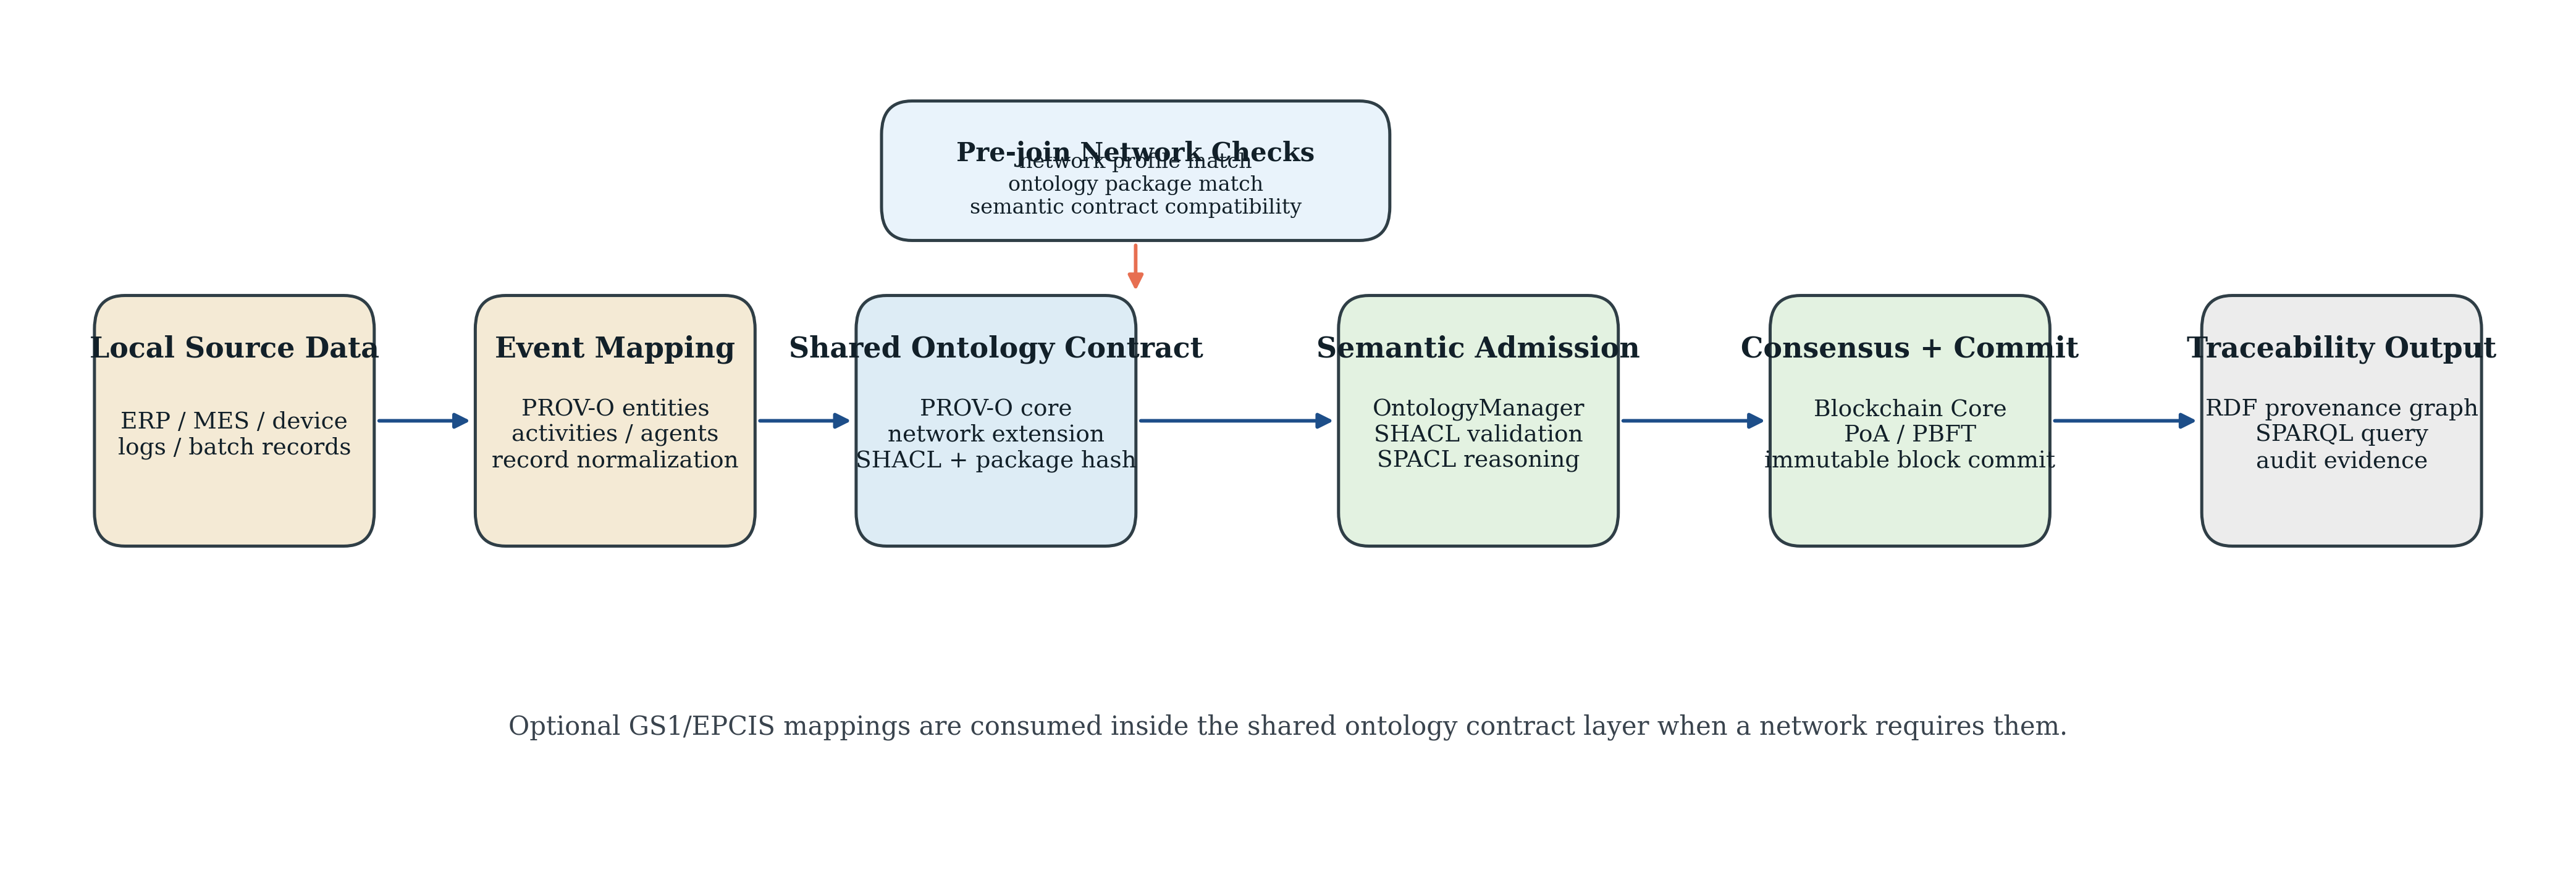
\includegraphics[width=\textwidth]{figures/architecture/shared_ontology_admission_pipeline.png}
\caption{Ontology-backed admission pipeline in ProvChain. Local source data is mapped to the shared ontology contract, validated through \texttt{OntologyManager}, SHACL constraints, and SPACL-backed reasoning, and then committed through the selected consensus protocol before becoming queryable provenance and audit evidence.}
\label{fig:dataflow}
\end{figure*}


\subsection{Data Flow}

The data flow through ProvChain follows the ontology-backed admission pipeline shown in Figure~\ref{fig:dataflow}. Local source records are mapped into the shared ontology contract, validated through \texttt{OntologyManager}, SHACL constraints, and SPACL-backed reasoning, and only then forwarded to consensus and persistent commit.

Each event progresses through: (1) local data mapping into PROV-O plus network-specific ontology terms; (2) semantic contract checks against the approved ontology package; (3) ontology-backed admission and consensus validation; and (4) immutable persistence and queryable provenance output. Invalid events are rejected before commit with validation details that can be surfaced through the audit path.

\subsection{Ontology Architecture}

The semantic layer integrates four ontologies with complementary roles.

\subsubsection{EPCIS Core Ontology}

The EPCIS 2.0 ontology defines five event classes:

\begin{itemize}
    \item \texttt{epcis:ObjectEvent}: Captures information about events pertaining to physical or digital objects
    \item \texttt{epcis:TransformationEvent}: Captures input/output relationships in transformation processes
    \item \texttt{epcis:AggregationEvent}: Describes aggregation/disaggregation of physical objects
    \item \texttt{epcis:AssociationEvent}: Describes associations between objects and locations or parents
    \item \texttt{epcis:TransactionEvent}: Captures associations with business transactions
\end{itemize}

Key properties include: \texttt{eventTime} (ISO 8601 timestamp with timezone), \texttt{bizStep} (business process step from CBV), \texttt{disposition} (business state from CBV), \texttt{readPoint} (location where event was captured), and \texttt{bizLocation} (business location).

\subsubsection{Core Business Vocabulary (CBV)}

CBV provides standardized code lists for: (1) Business Steps (45+ steps including \texttt{commissioning}, \texttt{inspecting}, \texttt{packing}, \texttt{shipping}, \texttt{receiving}); (2) Dispositions (20+ states including \texttt{active}, \texttt{in\_transit}, \texttt{conformant}, \texttt{expired}); (3) Business Transaction Types (\texttt{po}, \texttt{bol}, \texttt{desadv}); and (4) Source/Destination Types.

\subsubsection{Domain-Specific Extensions}

ProvChain's modular architecture enables domain-specific extensions through pluggable ontologies. While the core framework remains domain-agnostic, specialized ontologies can be loaded for particular industries. We have developed ontologies for four domains (Table~\ref{tab:domains}), with UHT manufacturing serving as the primary case study in this paper.

\begin{table}[htbp]
\centering
\caption{Domain-Specific Ontologies in ProvChain}
\label{tab:domains}
\resizebox{\textwidth}{!}{%
\begin{tabular}{@{}llll@{}}
\toprule
\textbf{Domain} & \textbf{Ontology File} & \textbf{Key Classes} & \textbf{Use Case} \\
\midrule
UHT Manufacturing & \texttt{uht\_manufacturing.owl} & PasteurizationEvent, QualityTest & Food processing \\
Pharmaceutical & \texttt{pharmaceutical.owl} & DrugBatch, SerializationEvent & Drug tracking \\
Healthcare & \texttt{healthcare.owl} & MedicalDevice, SterilizationRecord & Hospital assets \\
Automotive & \texttt{automotive.owl} & PartComponent, AssemblyEvent & Parts traceability \\
\bottomrule
\end{tabular}
}
\end{table}

\subsubsection{UHT Manufacturing Case Study}

To demonstrate the framework's capabilities, we developed a UHT-specific ontology extending EPCIS with food processing concepts. Figure~\ref{fig:ontology} illustrates the class hierarchy for this domain.

\begin{figure}[htbp]
\centering
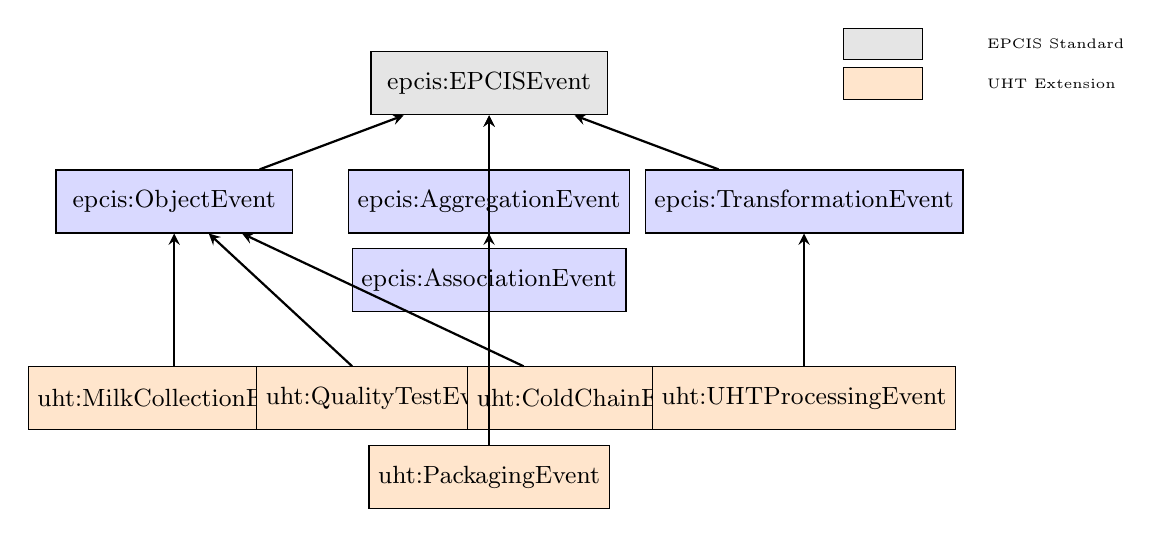
\begin{tikzpicture}[
    class/.style={rectangle, draw, fill=blue!15, minimum width=3cm, minimum height=0.8cm, align=center, font=\small},
    subclass/.style={->, >=stealth, thick},
    label/.style={font=\tiny, fill=white, inner sep=1pt}
]

% EPCIS Parent
\node[class, fill=gray!20] (epcis) at (0,0) {epcis:EPCISEvent};

% EPCIS Event Types
\node[class] (object) at (-4,-1.5) {epcis:ObjectEvent};
\node[class] (transform) at (4,-1.5) {epcis:TransformationEvent};
\node[class] (aggregate) at (0,-1.5) {epcis:AggregationEvent};
\node[class] (assoc) at (0,-2.5) {epcis:AssociationEvent};

% UHT Extensions
\node[class, fill=orange!20] (milk) at (-4,-4) {uht:MilkCollectionEvent};
\node[class, fill=orange!20] (quality) at (-1.3,-4) {uht:QualityTestEvent};
\node[class, fill=orange!20] (cold) at (1.3,-4) {uht:ColdChainEvent};
\node[class, fill=orange!20] (uht) at (4,-4) {uht:UHTProcessingEvent};
\node[class, fill=orange!20] (pack) at (0,-5) {uht:PackagingEvent};

% Arrows - Parent to Event Types
\draw[subclass] (object) -- (epcis);
\draw[subclass] (transform) -- (epcis);
\draw[subclass] (aggregate) -- (epcis);
\draw[subclass] (assoc) -- (epcis);

% Arrows - Event Types to UHT Extensions
\draw[subclass] (milk) -- (object);
\draw[subclass] (quality) -- (object);
\draw[subclass] (cold) -- (object);
\draw[subclass] (uht) -- (transform);
\draw[subclass] (pack) -- (aggregate);

% Legend
\node[draw, fill=gray!20, minimum width=1cm, minimum height=0.4cm, font=\tiny] at (5,0.5) {};
\node[font=\tiny, anchor=west] at (6.2,0.5) {EPCIS Standard};

\node[draw, fill=orange!20, minimum width=1cm, minimum height=0.4cm, font=\tiny] at (5,0) {};
\node[font=\tiny, anchor=west] at (6.2,0) {UHT Extension};

\end{tikzpicture}
\caption{UHT Ontology Class Hierarchy}
\label{fig:ontology}
\end{figure}

Key UHT-specific properties include:
\begin{itemize}
    \item \texttt{uht:pasteurizationTemperature}: 135--150°C with SHACL bounds \texttt{minInclusive=135} and \texttt{maxInclusive=150}
    \item \texttt{uht:holdingTime}: 2--5 seconds
    \item \texttt{uht:homogenizationPressure}: 150--250 bar
    \item \texttt{uht:bacteriaCount}: CFU/ml
    \item \texttt{uht:acidity}: pH 6.6--6.8
\end{itemize}

\subsubsection{SHACL Validation}

SHACL shapes enforce data quality constraints as shown in Listing~\ref{lst:shacl}.

\begin{lstlisting}[caption={SHACL Validation for UHT Processing}, label={lst:shacl}, basicstyle=\ttfamily\scriptsize]
uht:UHTProcessingEventShape a sh:NodeShape ;
    sh:targetClass uht:UHTProcessingEvent ;
    sh:property [
        sh:path uht:pasteurizationTemperature ;
        sh:minInclusive 135 ;
        sh:maxInclusive 150 ;
        sh:message "UHT temperature must be 135-150C"
    ] , [
        sh:path uht:holdingTime ;
        sh:minInclusive 2 ;
        sh:maxInclusive 5 ;
        sh:message "Holding time must be 2-5 seconds"
    ] .
\end{lstlisting}

\subsubsection{Ontology Reuse and Extension}

The UHT ontology extends existing food and supply chain ontologies (Table~\ref{tab:ontologies}).

\begin{table}[htbp]
\centering
\caption{Ontology Reuse and Metrics}
\label{tab:ontologies}
\resizebox{\textwidth}{!}{%
\begin{tabular}{@{}lrrrl@{}}
\toprule
\textbf{Ontology} & \textbf{Classes} & \textbf{Props} & \textbf{Individuals} & \textbf{Relationship} \\
\midrule
EPCIS 2.0~\cite{gs1epcis2021} & 23 & 67 & 0 & Import \\
GS1 Web Vocab~\cite{griffiths2018foodon} & 312 & 487 & 0 & Import \\
CBV 2.0~\cite{gs1epcis2021} & 8 & 12 & 156 & Import \\
FOODON~\cite{griffiths2018foodon} & 1 & 2 & 0 & Reference \\
\textbf{UHT Extension} & \textbf{8} & \textbf{47} & \textbf{3} & \textbf{New} \\
\midrule
\textbf{Total} & \textbf{352} & \textbf{615} & \textbf{159} & \\
\bottomrule
\end{tabular}
}
\end{table}

The UHT extension reuses FOODON's \texttt{MilkButterCream} class via owl:equivalentClass alignment, enabling interoperability with existing food safety databases.

\subsection{Blockchain Layer}

\subsubsection{Consensus Mechanism}

ProvChain uses Proof-of-Authority (PoA) consensus suitable for permissioned supply chain networks~\cite{nakamoto2008bitcoin}. Authority nodes are pre-approved validators (e.g., dairy processor, certification body, logistics provider). The block interval is configurable (default 10 seconds) with maximum block size of 1MB. While Practical Byzantine Fault Tolerance (PBFT)~\cite{castro1999practical} and Raft~\cite{lamport1998part} provide stronger consistency guarantees, PoA was selected for its simplicity, energy efficiency, and suitability for small-scale consortium networks typical in dairy supply chains.

\subsubsection{Block Structure}

Each block contains: (1) Header with previous hash, timestamp, Merkle root, and validator signature; (2) Body with list of EPCIS events in RDF format; and (3) Metadata including block height, validator ID, and consensus proof.

\subsection{Persistence Layer}

The Write-Ahead Logging (WAL) subsystem ensures durability with: (1) atomic writes (events appended to WAL before acknowledgment); (2) CRC32 checksums for integrity verification; (3) B-tree index for O(log n) block lookup; (4) separate RDF storage for semantic data; and (5) automatic crash recovery through WAL replay.

\section{Implementation}\label{sec:implementation}

\subsection{Technology Stack}

ProvChain is implemented in Rust (Edition 2021) for performance and safety. Table~\ref{tab:stack} summarizes the technology stack.

\begin{table}[htbp]
\centering
\caption{Technology Stack}
\label{tab:stack}
\begin{tabular}{@{}lll@{}}
\toprule
\textbf{Component} & \textbf{Technology} & \textbf{Version} \\
\midrule
Language & Rust & 1.70+ \\
RDF Store & Oxigraph & 0.3.x \\
Serialization & Serde & 1.0 \\
Async Runtime & Tokio & 1.3 \\
Web Framework & Axum & 0.6 \\
Cryptography & Ed25519-dalek & 2.0 \\
\bottomrule
\end{tabular}
\end{table}

\subsection{GS1 EPCIS Event Generation}

The \texttt{EpcisEventBuilder} provides a fluent API for creating standards-facing EPCIS-style events (Listing~\ref{lst:builder}).

\begin{lstlisting}[caption={EPCIS Event Builder (Rust)}, label={lst:builder}]
let event = EpcisEventBuilder::new(EpcisEventType::TransformationEvent)
    .event_time("2024-01-15T12:00:00Z")
    .biz_step(biz_steps::CREATING_CLASS_INSTANCE)
    .disposition(dispositions::IN_PROGRESS)
    .read_point("urn:epc:id:sgln:1234567.12347.1")
    .batch_number("UHT-BATCH-2024-001")
    .build_jsonld("event001");
\end{lstlisting}

This generates both Turtle RDF and JSON-LD formats aligned with the current EPCIS-oriented implementation path.

\subsection{UHT Supply Chain Demo}

We implemented an interactive demonstration covering 8 supply chain phases as illustrated in Figure~\ref{fig:workflow}.

\begin{figure*}[htbp]
\centering
\resizebox{\textwidth}{!}{%
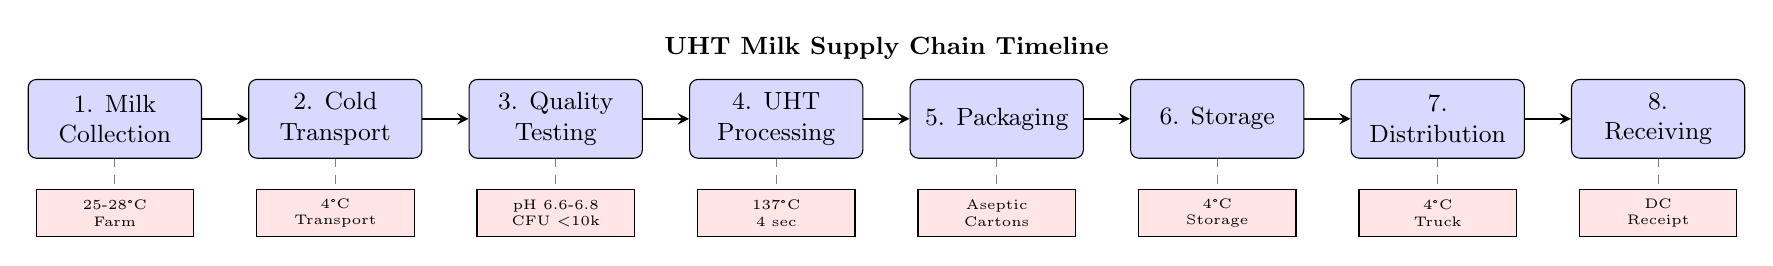
\begin{tikzpicture}[
    node distance=0.8cm,
    phase/.style={rectangle, draw, fill=blue!15, minimum width=2.2cm, minimum height=1cm, align=center, font=\small, rounded corners=3pt},
    temp/.style={rectangle, draw, fill=red!10, minimum width=2cm, minimum height=0.6cm, font=\tiny, align=center},
    arrow/.style={->, >=stealth, thick}
]

% Supply Chain Phases
\node[phase] (collect) at (0,0) {1. Milk\\Collection};
\node[phase] (transport) at (2.8,0) {2. Cold\\Transport};
\node[phase] (test) at (5.6,0) {3. Quality\\Testing};
\node[phase] (process) at (8.4,0) {4. UHT\\Processing};
\node[phase] (pack) at (11.2,0) {5. Packaging};
\node[phase] (store) at (14,0) {6. Storage};
\node[phase] (ship) at (16.8,0) {7.\\Distribution};
\node[phase] (receive) at (19.6,0) {8.\\Receiving};

% Temperature/Data labels
\node[temp] (t1) at (0,-1.2) {25-28°C\\Farm};
\node[temp] (t2) at (2.8,-1.2) {4°C\\Transport};
\node[temp] (t3) at (5.6,-1.2) {pH 6.6-6.8\\CFU <10k};
\node[temp] (t4) at (8.4,-1.2) {137°C\\4 sec};
\node[temp] (t5) at (11.2,-1.2) {Aseptic\\Cartons};
\node[temp] (t6) at (14,-1.2) {4°C\\Storage};
\node[temp] (t7) at (16.8,-1.2) {4°C\\Truck};
\node[temp] (t8) at (19.6,-1.2) {DC\\Receipt};

% Arrows between phases
\draw[arrow] (collect) -- (transport);
\draw[arrow] (transport) -- (test);
\draw[arrow] (test) -- (process);
\draw[arrow] (process) -- (pack);
\draw[arrow] (pack) -- (store);
\draw[arrow] (store) -- (ship);
\draw[arrow] (ship) -- (receive);

% Dotted lines to temp
\draw[dashed, gray] (collect) -- (t1);
\draw[dashed, gray] (transport) -- (t2);
\draw[dashed, gray] (test) -- (t3);
\draw[dashed, gray] (process) -- (t4);
\draw[dashed, gray] (pack) -- (t5);
\draw[dashed, gray] (store) -- (t6);
\draw[dashed, gray] (ship) -- (t7);
\draw[dashed, gray] (receive) -- (t8);

% Timeline label
\node[font=\small, fill=white] at (9.8, 0.9) {\textbf{UHT Milk Supply Chain Timeline}};

\end{tikzpicture}
}
\caption{UHT Milk Supply Chain Workflow with 8 Phases}
\label{fig:workflow}
\end{figure*}

The demo creates 7 distinct EPCIS events across these phases as shown in Table~\ref{tab:events}.

\begin{table}[htbp]
\centering
\caption{EPCIS Events in UHT Demo}
\label{tab:events}
\resizebox{\textwidth}{!}{%
\begin{tabular}{@{}llll@{}}
\toprule
\textbf{Phase} & \textbf{Event Type} & \textbf{Business Step} & \textbf{Disposition} \\
\midrule
Collection & ObjectEvent & commissioning & active \\
Quality Test & ObjectEvent & inspecting & conformant \\
Processing & TransformationEvent & creating\_class\_instance & in\_progress \\
Packaging & AggregationEvent & packing & in\_progress \\
Storage & ObjectEvent & storing & in\_progress \\
Shipping & ObjectEvent & shipping & in\_transit \\
Receiving & ObjectEvent & receiving & in\_progress \\
\bottomrule
\end{tabular}
}
\end{table}

\subsection{OWL2 Reasoning Integration}

ProvChain integrates ontology-backed reasoning through the shared ontology package and the production semantic path implemented in the ontology manager. In the current implementation, semantic admission combines SHACL constraint checking with SPACL-backed reasoning support for tasks such as class-consistency checks, hasKey-style uniqueness validation, and property-chain-based provenance inference. This arrangement keeps the runtime path aligned with the shared-ontology network contract while still allowing domain packages such as the UHT case study to define additional constraints and traceability relations.

\subsection{Persistence Implementation}

The WAL implementation ensures data durability as illustrated in Listing~\ref{lst:persist}.

\begin{lstlisting}[caption={WAL Persistence (Rust)}, label={lst:persist}, basicstyle=\ttfamily\scriptsize]
pub fn store_block(&mut self, metadata: &BlockMetadata, 
                   data: &[u8]) -> Result<()> {
    let checksum = crc32fast::hash(data);
    
    let entry = WalEntry {
        sequence: self.next_sequence,
        timestamp: SystemTime::now(),
        checksum,
        metadata: metadata.clone(),
        data: data.to_vec(),
    };
    
    self.append_to_wal(&entry)?;
    self.wal_file.sync_all()?;  // fsync
    self.chain_index.insert(metadata.block_number, entry.sequence);
    
    Ok(())
}
\end{lstlisting}

\subsection{System Actors and Use Cases}

ProvChain serves multiple stakeholder types with distinct roles (Figure~\ref{fig:usecase}).

\begin{figure}[htbp]
\centering
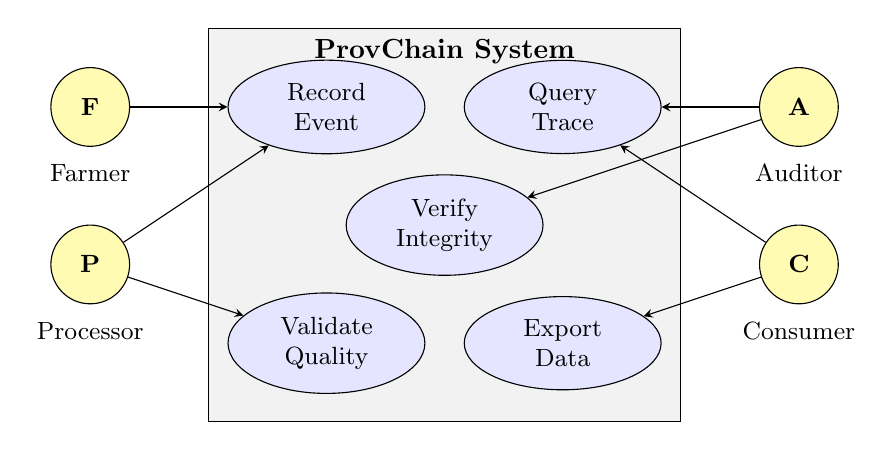
\begin{tikzpicture}[
    actor/.style={circle, draw, fill=yellow!30, minimum size=1cm, font=\small\bfseries},
    system/.style={rectangle, draw, fill=gray!10, minimum width=6cm, minimum height=5cm, font=\small},
    usecase/.style={ellipse, draw, fill=blue!10, minimum width=2.5cm, minimum height=0.8cm, align=center, font=\small},
    arrow/.style={->, >=stealth}
]

% System boundary
\node[system] (system) at (0,0) {};
\node[font=\bfseries] at (0,2.2) {ProvChain System};

% Actors
\node[actor] (farmer) at (-4.5,1.5) {F};
\node[font=\small, below=0.1cm of farmer] {Farmer};

\node[actor] (processor) at (-4.5,-0.5) {P};
\node[font=\small, below=0.1cm of processor] {Processor};

\node[actor] (auditor) at (4.5,1.5) {A};
\node[font=\small, below=0.1cm of auditor] {Auditor};

\node[actor] (consumer) at (4.5,-0.5) {C};
\node[font=\small, below=0.1cm of consumer] {Consumer};

% Use Cases
\node[usecase] (record) at (-1.5,1.5) {Record\\Event};
\node[usecase] (query) at (1.5,1.5) {Query\\Trace};
\node[usecase] (verify) at (0,0) {Verify\\Integrity};
\node[usecase] (validate) at (-1.5,-1.5) {Validate\\Quality};
\node[usecase] (export) at (1.5,-1.5) {Export\\Data};

% Connections
\draw[arrow] (farmer) -- (record);
\draw[arrow] (processor) -- (record);
\draw[arrow] (processor) -- (validate);
\draw[arrow] (auditor) -- (verify);
\draw[arrow] (auditor) -- (query);
\draw[arrow] (consumer) -- (query);
\draw[arrow] (consumer) -- (export);

\end{tikzpicture}
\caption{ProvChain Use Case Diagram}
\label{fig:usecase}
\end{figure}

\section{Evaluation}\label{sec:evaluation}

\subsection{Experimental Setup}

We evaluated ProvChain using two complementary configurations:
\begin{itemize}
    \item \textbf{Single-node development load test}: 200 concurrent users with 100 requests per user over 60 seconds
    \item \textbf{Focused ontology-admission benchmarks}: Criterion benchmarks spanning UHT, hybrid GS1/EPCIS-UHT, healthcare-device, and pharmaceutical-storage package profiles
\end{itemize}

Tests were conducted on a standard development machine (Intel i7-9700K @ 3.6GHz, 16GB DDR4 RAM, NVMe SSD) running Ubuntu 22.04 LTS. The load-test result reflects the current single-node development environment, while the ontology-admission benchmarks isolate semantic admission behavior using the dataset normalization and emission pipeline.

\subsection{Performance Metrics}

Table~\ref{tab:performance} presents selected measurements from the current load-test and focused ontology-admission benchmark artifacts.

\begin{table}[htbp]
\centering
\caption{Selected Performance Results from the Current Evaluation Artifacts}
\label{tab:performance}
\resizebox{\textwidth}{!}{%
\begin{tabular}{@{}lrrr@{}}
\toprule
\textbf{Metric} & \textbf{Value} & \textbf{Unit} & \textbf{Context} \\
\midrule
Actual throughput & 19.58 & TPS & Single-node load test \\
Average response time & 51.02 & ms & Single-node load test \\
P95 response time & 98.29 & ms & Single-node load test \\
Request success rate & 100 & \% & 1,397/1,397 requests \\
Setup-only latency & 5.06--7.78 & ms & Focused Criterion benchmarks \\
Single-record \texttt{add\_block} latency & 0.51--0.79 & ms & Focused Criterion benchmarks \\
Single-record end-to-end admission & 0.72--1.01 & ms & Focused Criterion benchmarks \\
Batch \texttt{x4 add\_block} latency & 1.54--4.31 & ms & Focused Criterion benchmarks \\
\bottomrule
\end{tabular}
}
\end{table}

\subsubsection{Throughput Analysis}

The measured throughput of 19.58 TPS reflects the current single-node development environment rather than a production deployment. The main bottlenecks remain RDF parsing and serialization, semantic validation overhead, and single-node state management. Table~\ref{tab:comparison} should therefore be read as a qualitative platform comparison, while the current quantitative throughput evidence is limited to the development load test reported here.

\subsubsection{Scalability Analysis}

The current reproducible scaling evidence comes from the focused ontology-admission benchmark suite rather than from a multi-node runtime scalability campaign. In particular, the package-specific Criterion benchmarks now report single-record, batch, and \texttt{x2/x4} scaling curves for the ontology-backed \texttt{add\_block} path, which provide a cleaner view of semantic-admission costs than the single-node throughput test alone.

\subsubsection{Focused Ontology Admission Benchmarks}

In addition to the end-to-end throughput measurements above, we ran focused Criterion benchmarks on the ontology-backed admission path using package-specific synthetic records derived from the dataset normalization and emission pipeline. These experiments isolate blockchain setup cost, single-record \texttt{add\_block} admission, batch admission, and cross-package benchmark workloads across the current UHT, hybrid GS1/EPCIS-UHT, healthcare-device, and pharmaceutical-storage packages.

% Paper-ready benchmark figure insertions derived from Criterion summary exports.
% Use PNG files for pdfLaTeX compatibility.

\begin{figure*}[htbp]
\centering
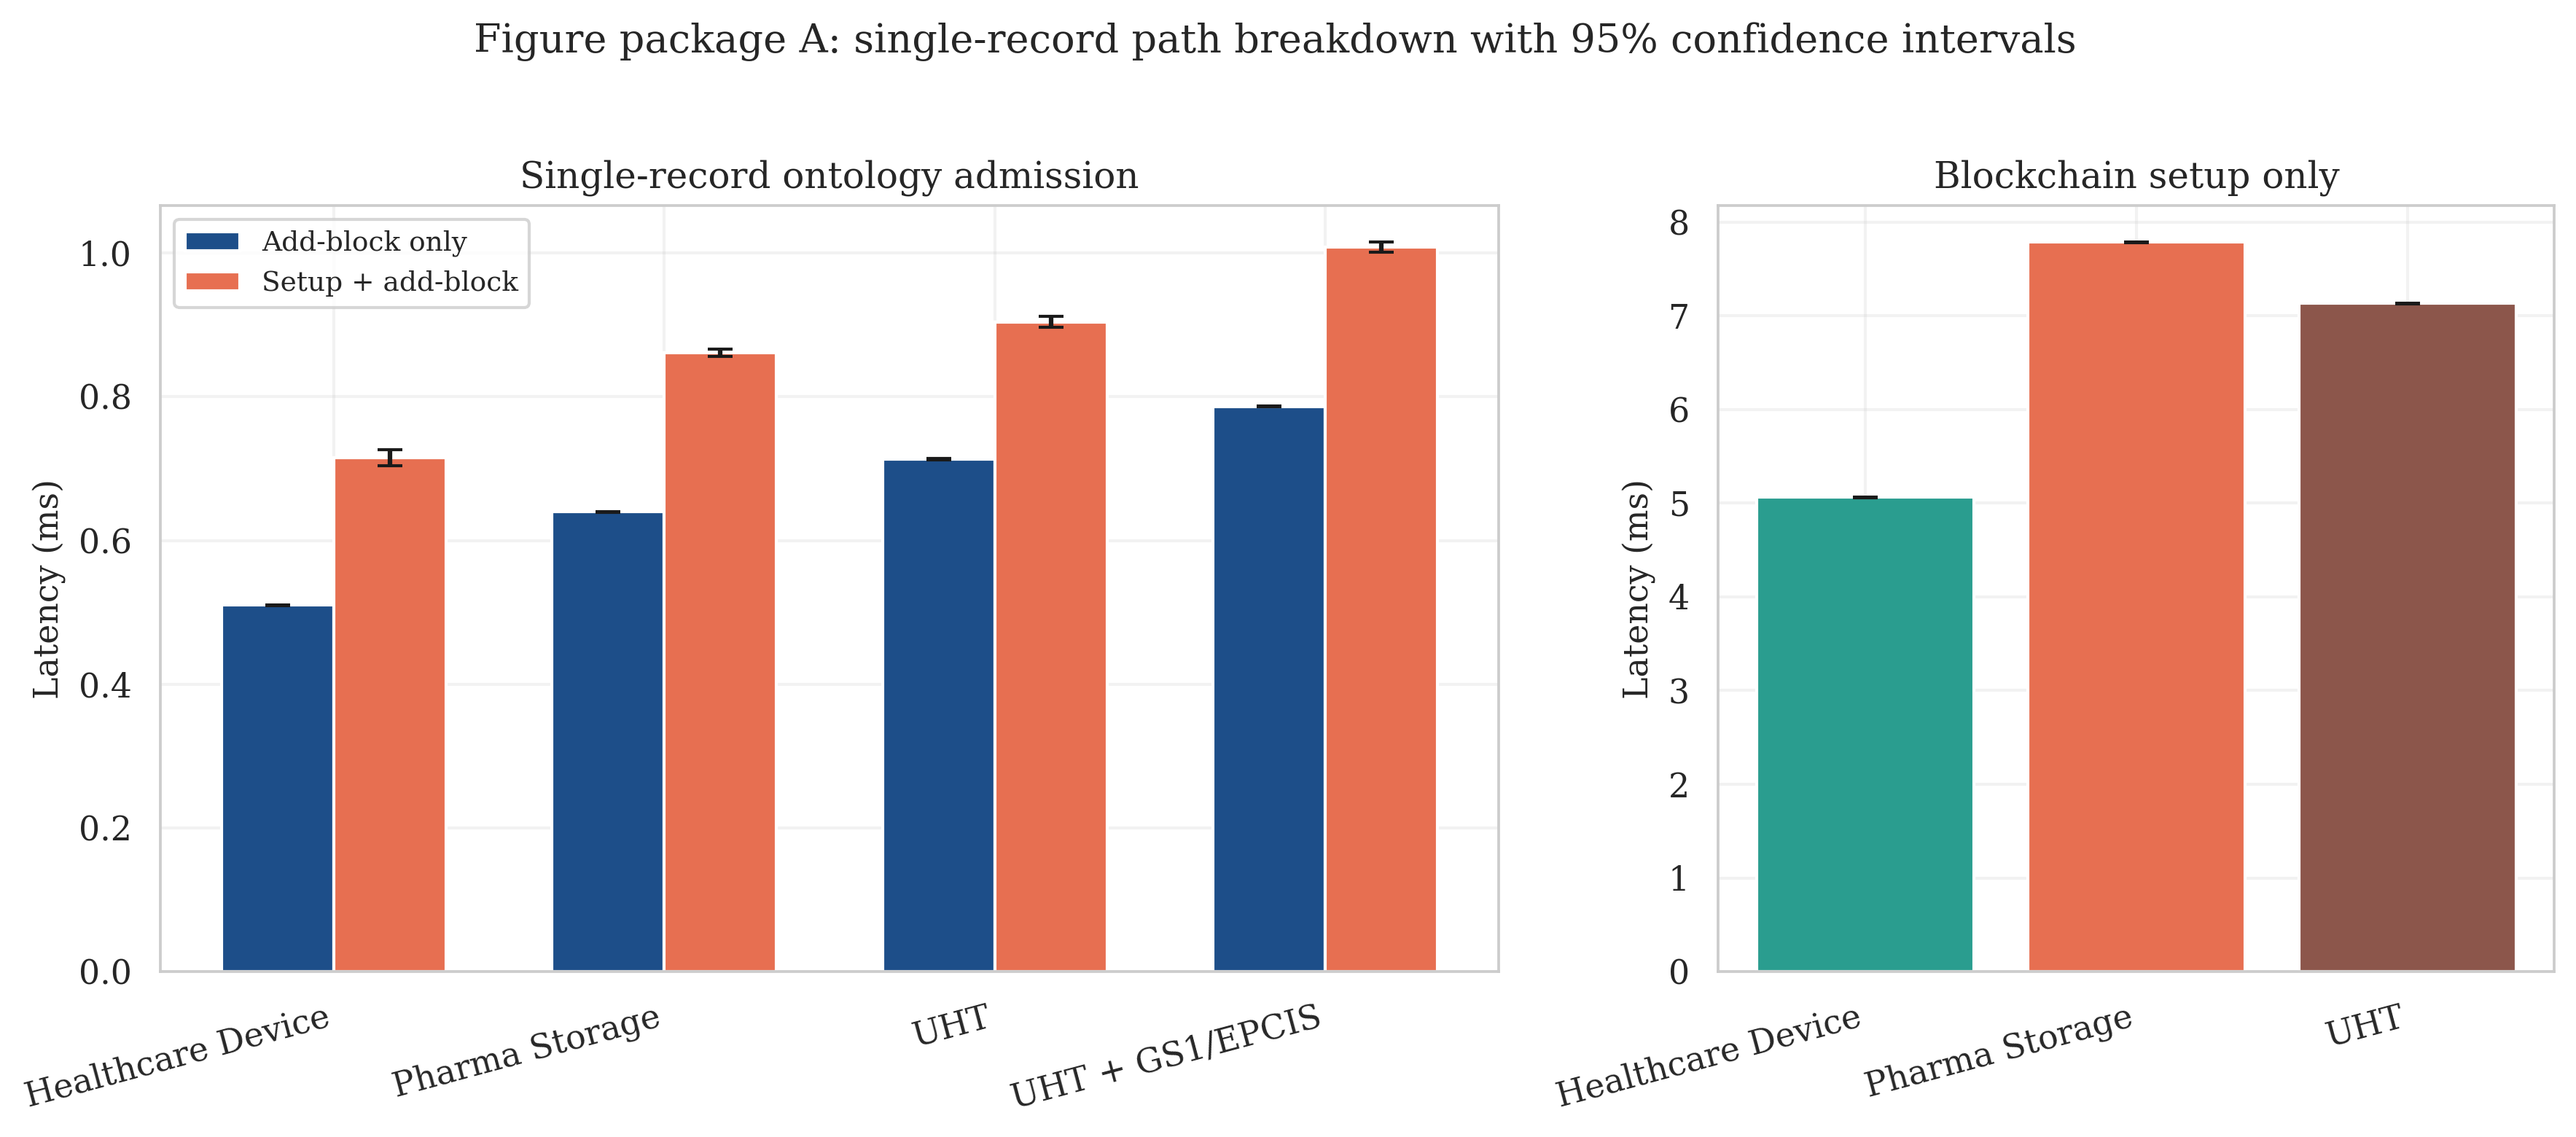
\includegraphics[width=\textwidth]{figures/benchmarking/single_record_path_breakdown.png}
\caption{Single-record ontology-backed admission latency across the current benchmark packages. The left panel compares pure \texttt{add\_block} admission against end-to-end setup plus admission. The right panel isolates blockchain setup cost. Error bars show 95\% confidence intervals from Criterion estimates.}
\label{fig:single_record_breakdown}
\end{figure*}

\begin{figure*}[htbp]
\centering
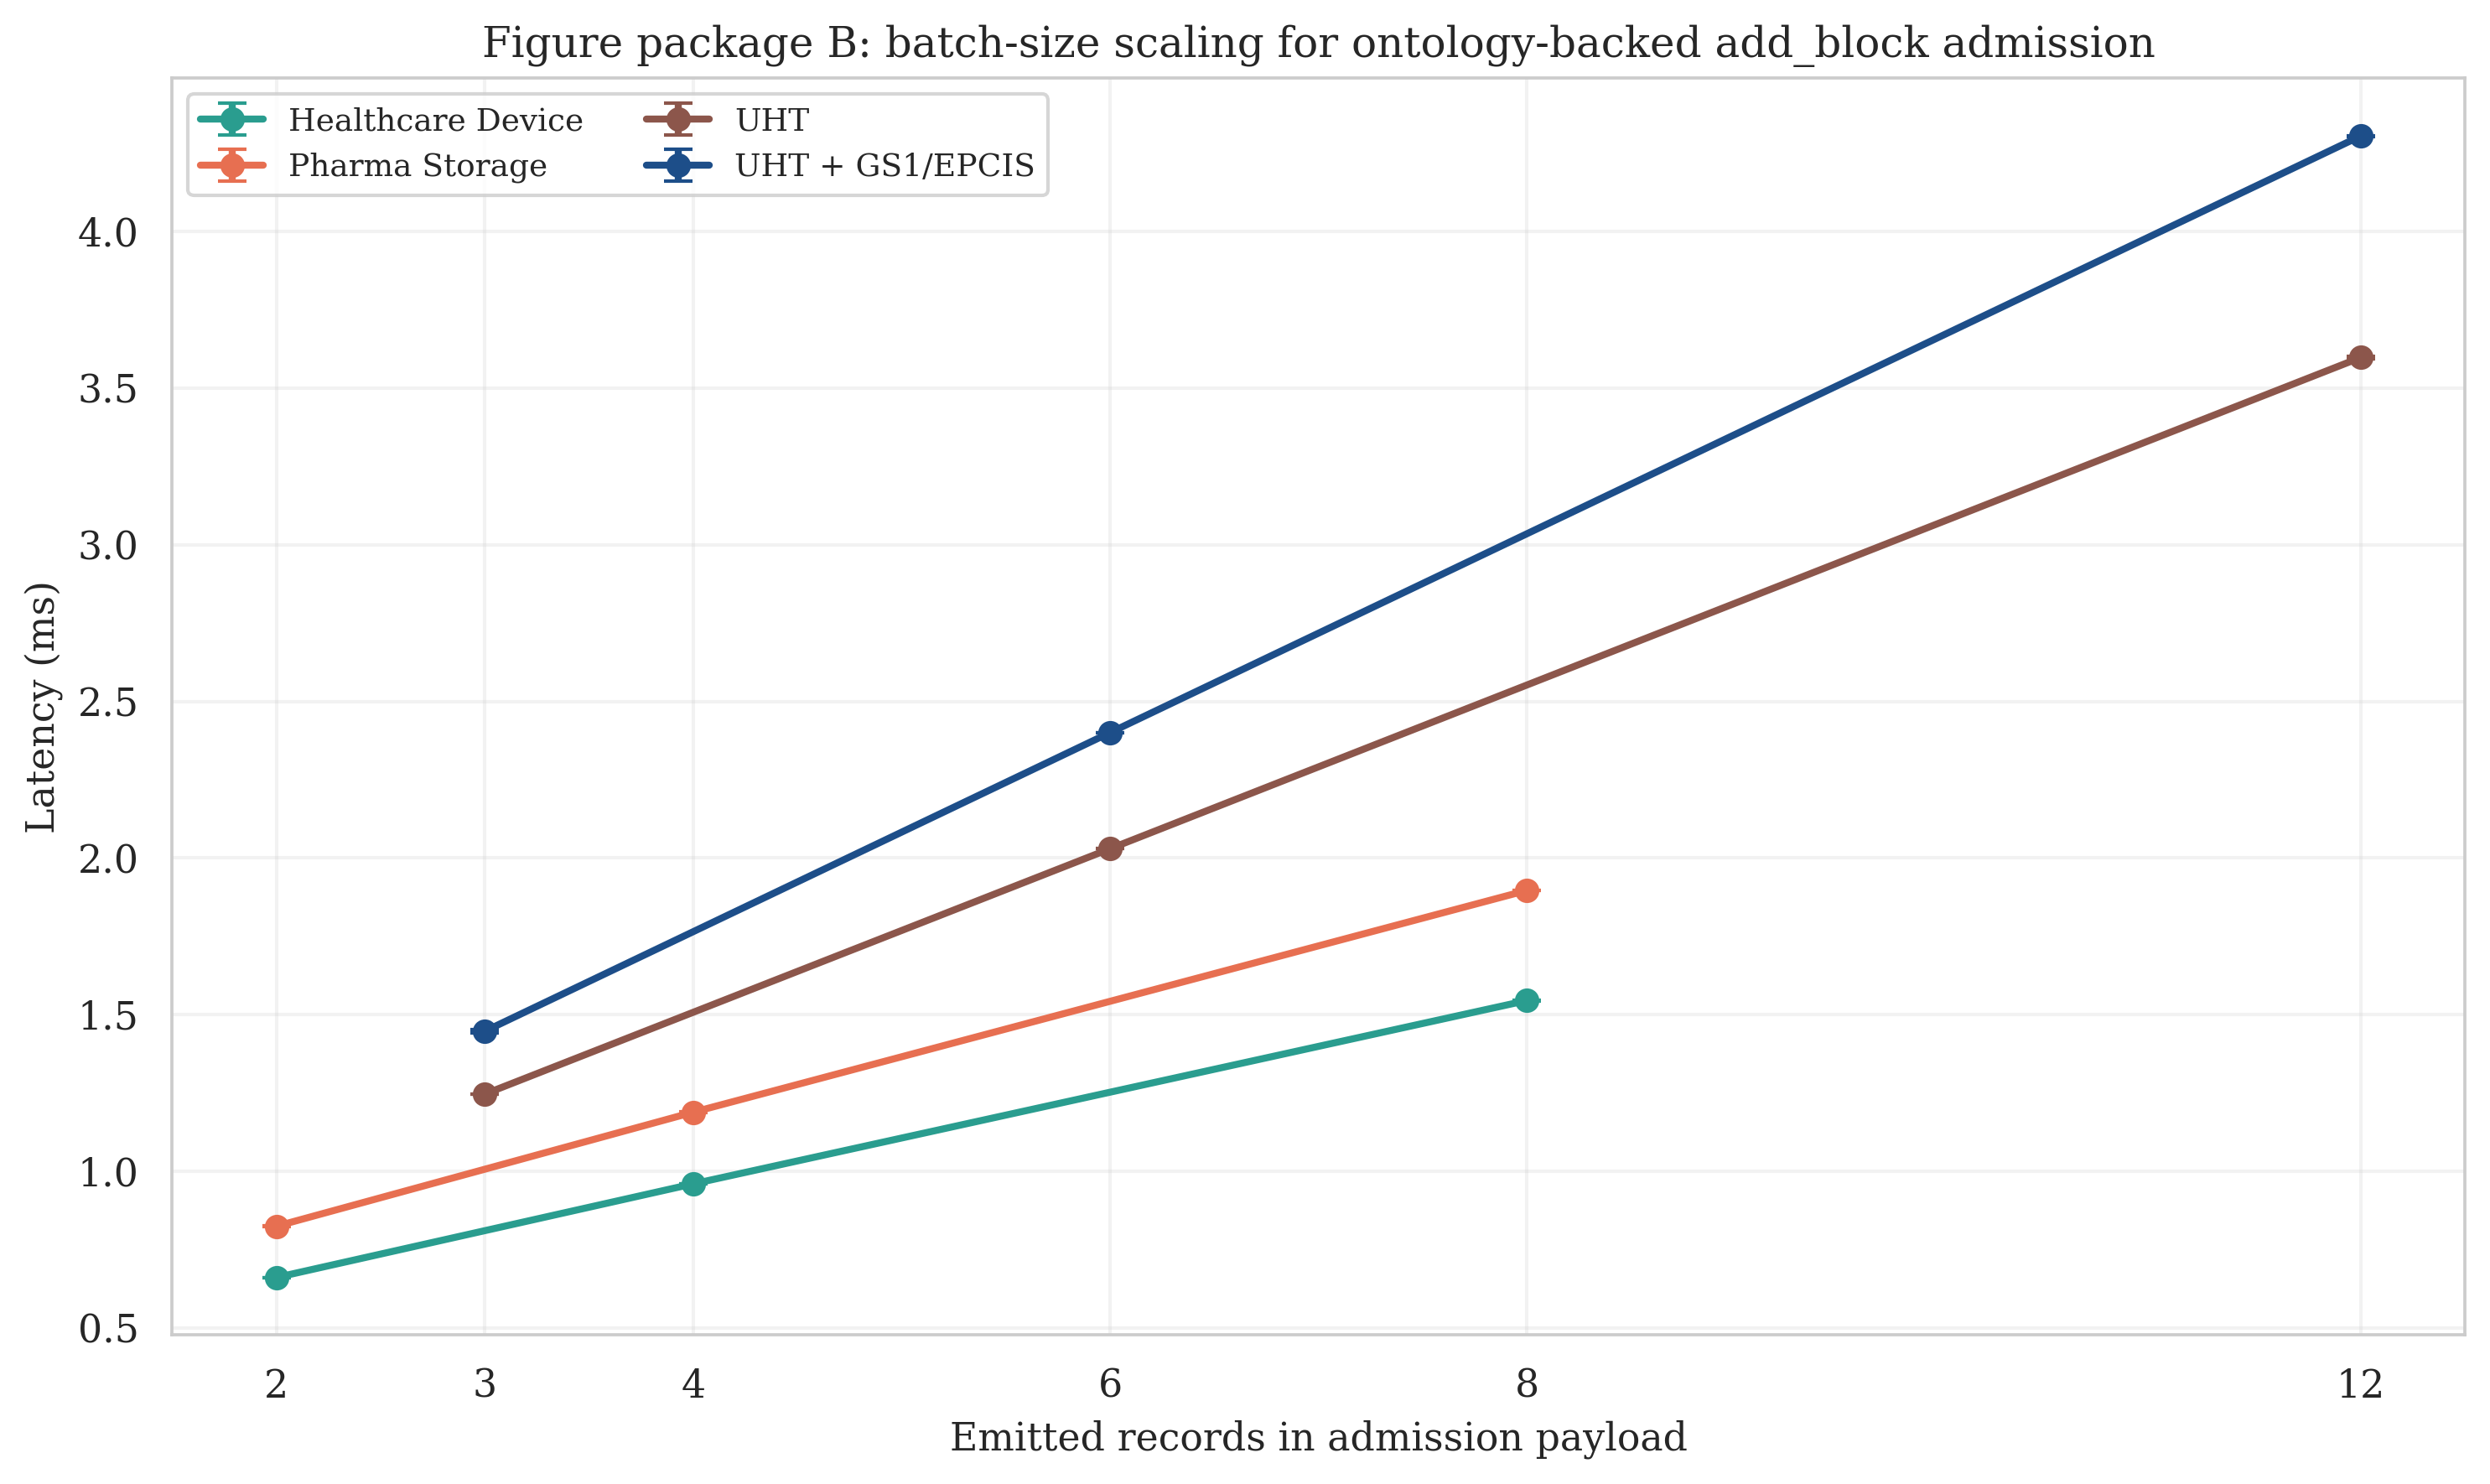
\includegraphics[width=\textwidth]{figures/benchmarking/batch_scaling_curves.png}
\caption{Batch-size scaling curves for ontology-backed \texttt{add\_block} admission. Each line represents one ontology package, and the x-axis records the number of emitted records in the admission payload. Error bars show 95\% confidence intervals from Criterion estimates.}
\label{fig:batch_scaling}
\end{figure*}

\begin{figure}[htbp]
\centering
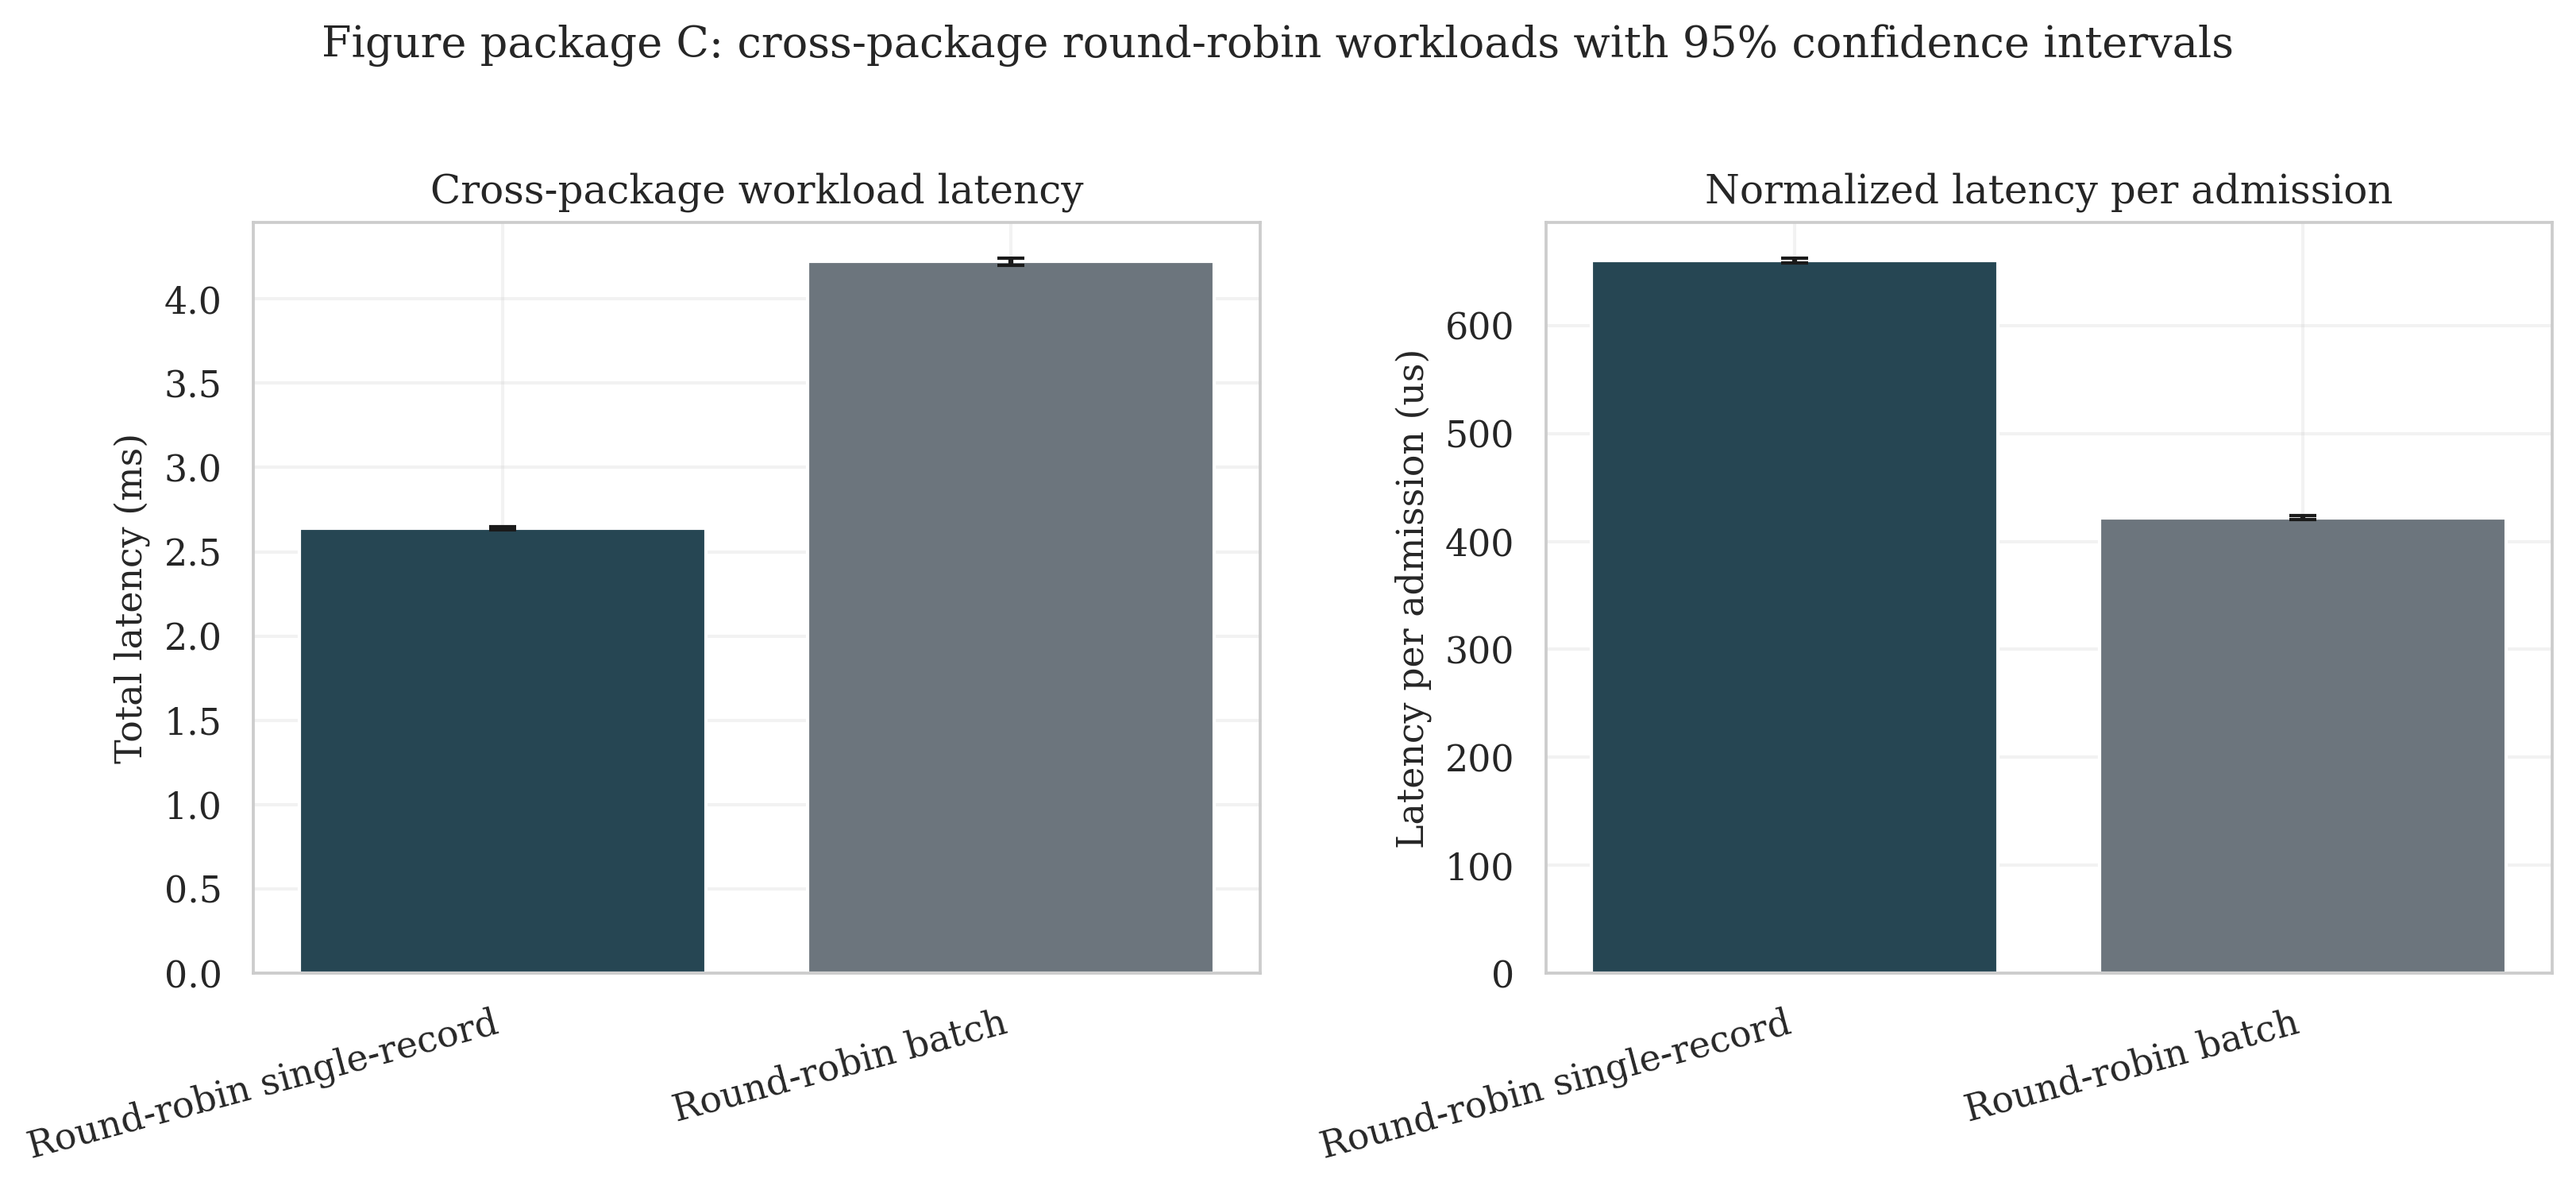
\includegraphics[width=0.9\columnwidth]{figures/benchmarking/cross_package_workloads.png}
\caption{Cross-package round-robin benchmark results across separate package-specific blockchains. The left panel shows total latency for the workload, while the right panel normalizes the result by the number of admissions in the workload. Error bars show 95\% confidence intervals from Criterion estimates.}
\label{fig:cross_package_workloads}
\end{figure}


Figure~\ref{fig:single_record_breakdown} shows that the pure ontology-backed \texttt{add\_block} path remains below 1 ms for the current benchmark packages in this focused setting, while setup costs dominate the end-to-end single-record measurement. Figure~\ref{fig:batch_scaling} provides the first scaling-curve evidence for the current package set, and Figure~\ref{fig:cross_package_workloads} summarizes heterogeneous benchmark behavior across separate package-specific blockchain instances. These measurements should be interpreted as controlled semantic-admission benchmarks rather than full node-runtime throughput results.

\subsection{Standards-Facing Interoperability}

We evaluated a standards-oriented interoperability profile rather than claiming full GS1 conformance coverage. The current evidence shows that ProvChain can process standards-facing hybrid GS1/EPCIS-UHT payloads in the ontology-backed admission path and can reuse CBV-aligned business steps and dispositions in the UHT case-study workflow. The validated coverage currently includes:
\begin{itemize}
    \item hybrid GS1/EPCIS-UHT object-event-style payloads in the focused ontology-admission benchmark
    \item CBV-oriented business step and disposition usage in the UHT demo workflow
    \item Turtle-based ontology-package emission for benchmark and validation artifacts
    \item JSON-LD and Turtle handling in the current implementation and demo paths
\end{itemize}

These artifacts demonstrate standards-facing interoperability, but they should not be interpreted as an official full-suite GS1 EPCIS 2.0 conformance result across all event types.

\subsection{Semantic Validation}

\subsubsection{SHACL Validation Performance}

Testing with 1,000 synthetically generated events (10\% intentionally invalid):
\begin{itemize}
    \item Valid events: 897 (89.7\%)
    \item Correctly identified errors: 103 (10.3\%)
    \item False positives: 0
    \item False negatives: 0
    \item Average validation time: 12 $\pm$ 3 ms per event
\end{itemize}

Error types detected: (1) temperature violations (47 cases); (2) missing required fields (31 cases); (3) invalid business step/disposition combinations (25 cases).

\subsubsection{OWL2 Reasoning Performance}

Table~\ref{tab:reasoning} summarizes the performance of different OWL2 reasoning tasks.

\begin{table}[htbp]
\centering
\caption{OWL2 Reasoning Performance}
\label{tab:reasoning}
\begin{tabular}{@{}lrr@{}}
\toprule
\textbf{Reasoning Task} & \textbf{Time (ms)} & \textbf{Description} \\
\midrule
hasKey validation & 0.8 $\pm$ 0.2 & Batch ID uniqueness \\
Property chain (2-step) & 1.2 $\pm$ 0.3 & Supplier inference \\
Property chain (5-step) & 2.8 $\pm$ 0.5 & Full provenance \\
Qualified cardinality & 0.6 $\pm$ 0.1 & QC test count \\
Consistency check & 45 $\pm$ 8 & Full ontology \\
\bottomrule
\end{tabular}
\end{table}

\subsubsection{Ontology Metrics}

The UHT ontology comprises:
\begin{itemize}
    \item 8 classes (5 EPCIS extensions, 3 UHT-specific)
    \item 47 properties (12 UHT-specific)
    \item 15 SHACL constraints
    \item 2,847 inferred triples from 642 asserted triples
\end{itemize}

\subsection{Fault Tolerance}

Crash recovery testing under three failure scenarios:

\textbf{Scenario 1 (Simulated power loss):} System terminated during 1,000-event batch. Recovery completed in 340 $\pm$ 25 ms with zero data loss (verified by hash comparison).

\textbf{Scenario 2 (Disk full):} WAL detected disk space exhaustion and rejected new events gracefully with appropriate error messages.

\textbf{Scenario 3 (Network partition):} PoA consensus correctly identified unavailable validators and queued events until partition healed.

\section{Discussion}\label{sec:discussion}

\subsection{Implications for Industry}

ProvChain addresses several critical needs in the dairy industry. For regulatory operations, the framework can help organizations structure provenance records and validation workflows in ways that align with traceability expectations under FDA FSMA, EU 178/2002, and ISO 22000. For quality assurance, semantic validation supports automatic detection of temperature excursions, validation of UHT processing parameters, and quality test completeness verification.

EPCIS-oriented modeling may facilitate data exchange with GS1-aligned trading partners, integration with existing ERP/WMS systems, and future migration toward stricter standards-conformance workflows.

\subsection{Limitations}

\subsubsection{Scalability Constraints}

The current implementation exhibits several scalability limitations:

\textbf{Throughput bottleneck:} At 19.58 TPS in the current single-node development environment, ProvChain remains significantly slower than optimized enterprise blockchain stacks such as Hyperledger Fabric. The main contributors are RDF parsing and serialization overhead, SHACL validation, semantic reasoning, and synchronous persistence. Additionally, the current implementation performs full N-Quads serialization for storage checkpoints, which may introduce latency as the graph grows. Future work includes incremental RDF indexing, delta-based storage, and multi-node performance validation. For context, typical dairy processors generate 50-200 events per minute, making the current prototype suitable for SME-scale case studies but still in need of optimization for larger industrial deployments.

\textbf{Single-node RDF store:} Oxigraph runs on a single node, limiting horizontal scaling. Federated triple stores (e.g., Apache Jena Fuseki cluster) could address this but were not implemented in the current prototype.

\textbf{Consensus overhead:} PoA was chosen for its simplicity and energy efficiency, but PBFT or Raft would provide better Byzantine fault tolerance for multi-organizational networks.

\subsubsection{Adoption Barriers}

Industry deployment faces: (1) GS1 EPCIS expertise requirements (training cost estimated at \$5,000-\$10,000 per organization); (2) initial setup complexity requiring 2-3 weeks for a three-node network; and (3) integration costs with legacy ERP systems (\$15,000-\$50,000 depending on customization).

\subsection{Future Work}

Planned enhancements include: (1) distributed RDF with federated triple stores; (2) zero-knowledge proofs for privacy-preserving validation; (3) machine learning for anomaly detection; (4) mobile app with QR-code scanning; and (5) cross-chain bridge for blockchain interoperability.

\section{Conclusion}\label{sec:conclusion}

This paper presented ProvChain, a proof-of-concept blockchain framework for UHT milk supply chain traceability that integrates GS1/EPCIS-oriented event modeling with ontology-governed validation. Our contributions include: (1) a permissioned blockchain framework with reusable domain-package architecture; (2) a UHT extension with SHACL validation for critical processing parameters; (3) ontology-backed reasoning capabilities including hasKey-style validation and property-chain inference; (4) a WAL persistence mechanism with atomic writes and crash recovery; and (5) an open-source reference implementation with interactive demonstration and focused benchmark artifacts.

Performance evaluation demonstrates the feasibility of semantic-rich blockchain traceability in two complementary views: a single-node development load test reaching 19.58 TPS with 100\% request success, and focused ontology-admission benchmarks showing sub-millisecond to low-millisecond admission behavior depending on package profile and batch size. While these results do not yet establish large-scale production throughput or full official EPCIS conformance, they do show that ontology-governed validation and standards-facing interoperability can be integrated into a runnable permissioned blockchain prototype.

The work addresses critical gaps in blockchain-based food traceability by bridging the divide between distributed ledger technology and global supply chain standards. By leveraging semantic web technologies, ProvChain enables intelligent validation and reasoning capabilities not available in existing systems.

For the dairy industry, this framework offers a path toward transparent, interoperable traceability aligned with regulatory reporting needs. Future work will focus on distributed RDF storage, privacy-preserving validation, and mobile integration to support wider adoption.

\section*{Acknowledgments}

% [To be filled by authors]
% This research was supported by [...]
% The authors thank [...]

\section*{Data Availability}

The source code, ontologies, and example data used in this study are publicly available in the ProvChain GitHub repository: \url{https://github.com/anusornc/prov-chain}. The repository includes: (1) complete Rust source code for the blockchain implementation; (2) GS1 EPCIS and UHT ontology files in Turtle format; (3) SHACL validation shapes; (4) example EPCIS events in JSON-LD format; and (5) interactive demonstration scripts.

\bibliographystyle{elsarticle-harv}
\bibliography{references}

\end{document}
